\documentclass[10pt,twocolumn,letterpaper]{article}

\usepackage{iccv}
\usepackage{caption}
\usepackage{times, graphicx, amsmath, amssymb, subcaption}

% Include other packages here, before hyperref.

% If you comment hyperref and then uncomment it, you should delete
% egpaper.aux before re-running latex.  (Or just hit 'q' on the first latex
% run, let it finish, and you should be clear).
\usepackage[pagebackref=true,breaklinks=true,colorlinks,bookmarks=false]{hyperref}

%\iccvfinalcopy % *** Uncomment this line for the final submission

\def\iccvPaperID{1341} % *** Enter the ICCV Paper ID here
\def\httilde{\mbox{\tt\raisebox{-.5ex}{\symbol{126}}}}

% Pages are numbered in submission mode, and unnumbered in camera-ready
\ificcvfinal\pagestyle{empty}\fi
\begin{document}

%%%%%%%%% TITLE
\title{Mosaicing Quad-Copter Imagery Containing Empty Space}

\author{Meghshyam G. Prasad and Sharat Chandran\\
Dept of Computer Science \& Engineering, \\
Indian Institute of Technology Bombay\\
{\tt\small \{meghshyam, sharat \}@cse.iitb.ac.in }
% For a paper whose authors are all at the same institution,
% omit the following lines up until the closing ``}''.
% Additional authors and addresses can be added with ``\and'',
% just like the second author.
% To save space, use either the email address or home page, not both
\and
Michael S. Brown\\
School of Computing, NUS, Singapore\\
{\tt\small brown@comp.nus.edu.sg}
}

\maketitle
%\thispagestyle{empty}


%%%%%%%%% ABSTRACT
\begin{abstract}
This paper focuses on a method to construct panoramas captured from a quad-copter that 
consists of scenes with large regions of empty space.  These empty spaces yields little to no features to match between input images making them challenging for existing mosaicing techniques.  We describe a framework that is able to handle this unique input by leveraging the availability of the IMU data from the quad-copter that is synchronized with the input images.  Specifically, our method uses the accompanying IMU data to select a subset of images that contain interesting scene content.  These images are then grouped into subgraphs, again using the IMU data, that can be stitched into a series of  non-overlapping mini-panoramas.  The gaps of these mini-panoramas represent regions of empty spaces in the scene.  We again use the IMU data together with coarse stereo reconstruction to determine the appropriate images in the input sequence to use to fill in the empty spaces.  We demonstrate the efficacy of our approach on a number of input sequences that cannot to be mosaiced by existing methods.
\end{abstract}

%%%%%%%%% BODY TEXT
\section{Introduction}

Aligning input images, finding features, and then compositing these
images into ultra wide photographs is one of the success stories of
computer vision.  Virtually most recent consumer cameras have this
technology embedded.  The success of the method rely significantly in
finding common features in the images taken, and thereby identifying an
appropriate match.

Unfortunately several scenes contain situations when this process is
defeated.  In designs where patterns are repeated, the matching
algorithm may incorrectly conclude which portions of the images are to
be aligned. 
%Figure 1 shows an example of this. 
A more serious cause of concern is when the area to be imaged simply
does not contain features.  This sort of situation occur in a variety
of situations such as paintings in an art exhibition, or posters in an
auditorium.  Fig~\ref{fig:teaser} shows an example of this
case. 

Indeed, one can imagine other situations where the viewer would like
to stitch together pictures well separated with empty (in the mind of
the viewer) or void spaces between them.  Our goal in this paper is to
create a mosaic of panaromic imagery with `dead space';
by `dead space' we mean portions of the input where a computer vision
feature matching algorithm is defeated due to a high likelihood of
absence of features, or when features can get confused.

\begin{figure}[t!]
  \centering
  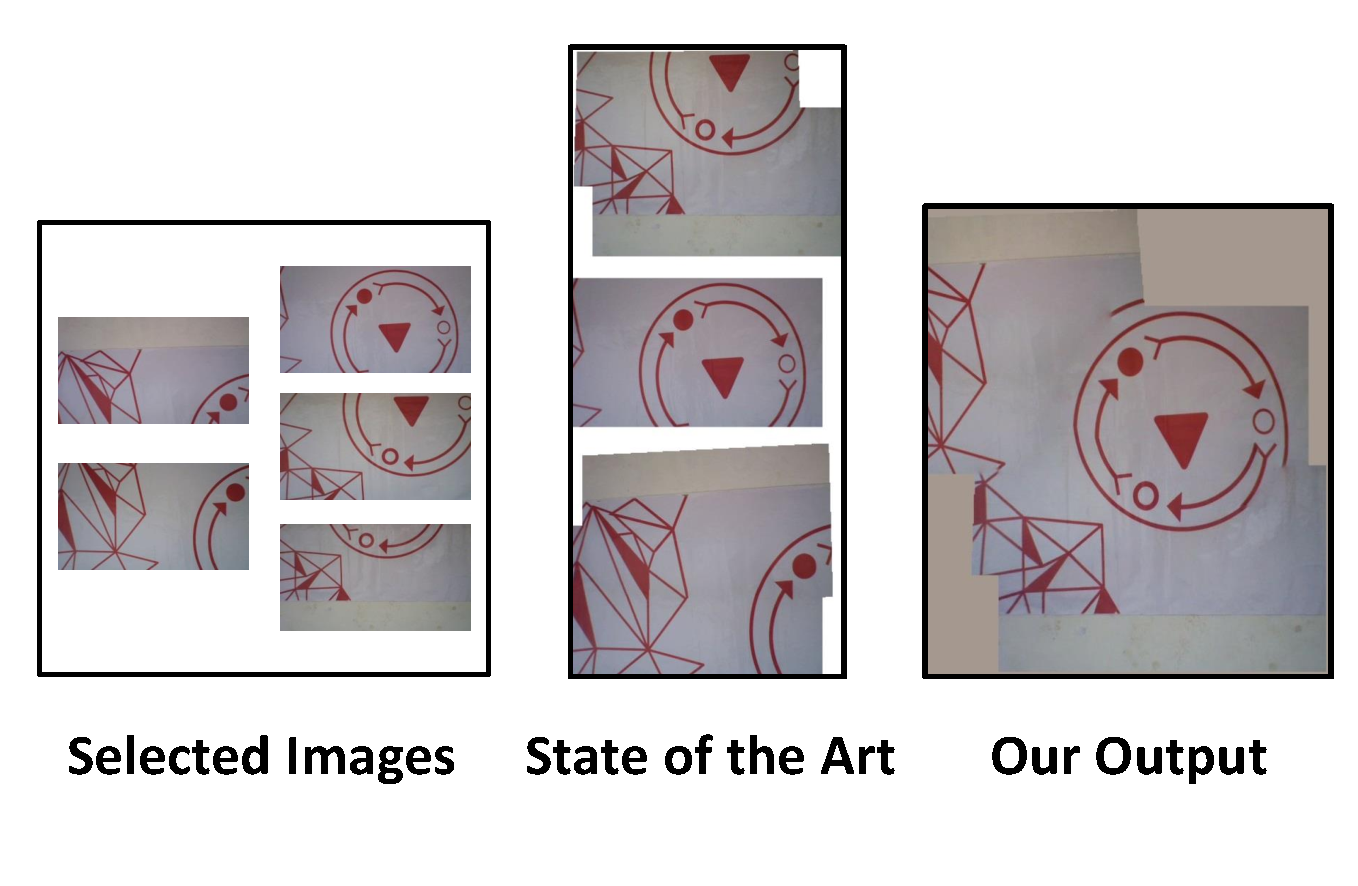
\includegraphics[width=0.49\textwidth]{figures/teaser1}
  \caption{ \label{fig:teaser} The ground truth picture shows a common
    situation in which dead space exists between large pictures (here,
    two poster boards). The input images (second column) show parts of
    the imagery obtained. Even if each of the images of the two
    individual posters can be stitched together (third column), the
    state of the art method encounter the dead space and is unable to
    make a complete mosaic.  It outputs either the first poster or the
    second, but not both together.  Our method (last column) succeeds
    since the imagery is acquired using a quadcopter that has
    positional information.}
\end{figure}

{\bf Key Idea} We propose to solve the dead space problem by using an
inexpensive off-the-shelf flying device, such as a quadcopter.  An
autonomous programmed quadcopter is particularly enticing because of
its ability to fly to areas that are accessible to the human eye, but
inaccessible for the human to reach.  Such areas do not lend
themselves easily to high quality orthographic images. Our solution
uses coarse positional information that a quadcopter can be assumed to
have.  The proximity relationship that the resultant images have can
be used to significantly reduce the search space.  Further, the
proximity relationship also allows to vary the parameters involved in
feature selection. For example, if there is reason to believe that two
images are adjacent horizontally, one can choose to adjust
thresholds in feature matching algorithm to hunt for otherwise elusive
matching pairs. 

{\bf Contributions} The main technical contribution of this paper is
that it improves the state of the art in mosaicing.  We assume that
the imagery is acquired by a quadcopter for the reasons mentioned
above. Sending a battery of images from a quadcopter to an image
mosaicing (alternatively, stitching) algorithm such as Autostitch
incapacitates the algorithm because of the sheer number of
images. Sending a sampled version of images to a manageable number $N$
of images, with $O(N^2)$ possible areas to match for features, also
does not work since the sampled image contains dead space.  In this
paper, we use positional information that lends itself to a graceful
$O(N)$ algorithm.  Some sample results are shown in Figure~\ref{fig:teaser}.
Other results are available in the experiments section and also in the
supplementary material.

{\bf Limitations} In this paper, we assume that the scene lies on a
planar surface, or can be deemed to lie on a planar surface. The
standard homography computation is still possible because of the dead
spaces.  We reduce the mosaicing problem to the stereo problem and are
thus able to complete the panorama.

The rest of this paper is organized as follows.  In the next section,
we discuss related work.  Subsequently we describe the main steps in
our process, and justify the process in Section~\ref{sec:results} with
experimental results.  The data and the code will be made available
later, but as of now it is available in the supplementary material.
The final section discusses future work.

\section{Related Work}

Panoramic image stitching or Image Mosaicing is well-studied problem in the
field of computer vision. Though it may not be possible to list all works,
(representatives include \cite{Milgram1975}, \cite{Milgram1977}, \cite{Capel},
\cite{Szeliski1997} \cite{Brown}, \cite{Brown07}), one may look
\cite{Szeliski05imagealignment} for a thorough survey.
Also, there are various freeware as well as commercial softwares available  for
performing image stitching, prominent ones are AutoStitch \cite{autostitch},
Microsoft’s Image Compositing Editor \cite{ICE}, and Adobe’s Photoshop CS6 \cite{photoshop}.

Gao et al. \cite{Gao} have used concept of ``Dual Homography'' to stitch
non-planar patches in images. Lhuillier et al.\cite{Lhuillier} have successfully
stitched images with motion parallax i.e., relief mosaics, using joint view triangulation. 
Acha et al. \cite{Acha} aligned dynamic scenes using notion of ``dynamics
constancy''. 

Agarwala et al.\cite{Agarwala2006} had used Markov Random Field (MRF)
optimization for stitching relatively sparse set of images captured using
handheld still camera which is moved along the scene. Eden et al. \cite{Eden}
were able to stitch images with large exposure difference as well as large
scene motion into single HDR quality image without using any additional camera hardware.

All of the image mosaicing methods works only when there is a
``intersection'' in feature space of images to be stitched. But, when there are
``gaps'' (either physical or due to lach of features) between images to be
stiched, we may have to use some other alignement method. In this paper, we use
stereo method to do alignement of images. Peleg et al. \cite{Peleg} have used
similar concept to create Stereo Panorama with a single camera.

\section{Methodology}

The goal of this paper is to compute a panorama of a scene lying on
one or many planar surfaces.  A schematic of two possible scenes for
this problem is shown in Figure~\ref{fig:schematic}.

\begin{figure}[h!]
  \centering
  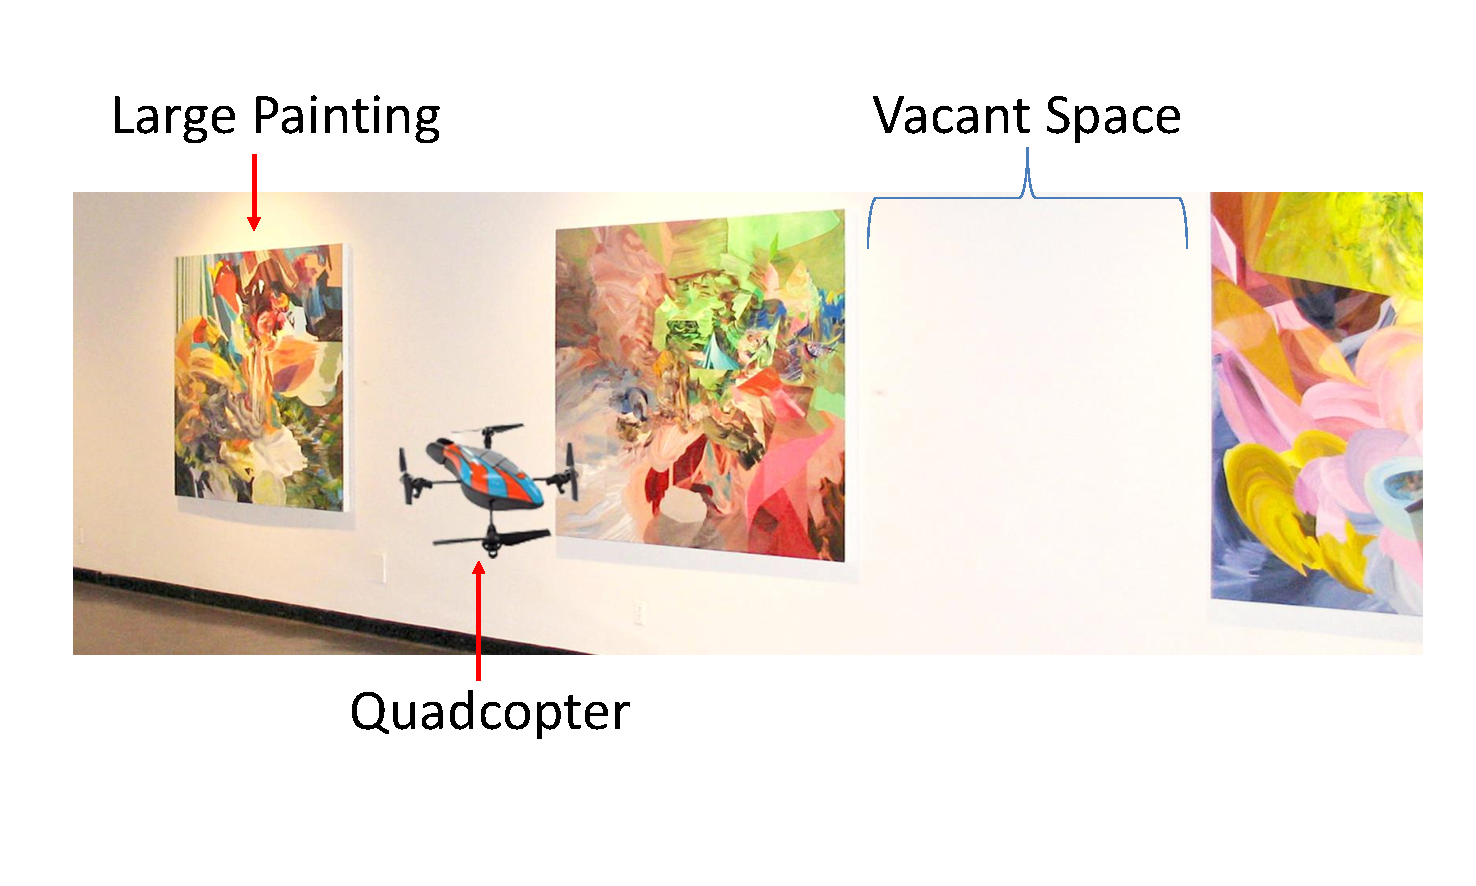
\includegraphics[width=0.49\textwidth]{figures/indoor}   
  \caption{ \label{fig:schematic} Problem definition: Dead space is
    encountered in varoious scenes.  When individual
    portions are captured by a quadcopter, how does one create the
    complete mosaic given that common features are either not
    available, or confusing?
  }
\end{figure}    

The method adopted consists of three steps described below. An
overview is shown in Figure~\ref{fig:workflow}.  In brief, we
systematically acquire a video of the scene, reduce the large number
of images into a manageable number, and finally mashup the images
acquired from different positions into a mosaic.

\begin{figure}[b!]
  \centering
  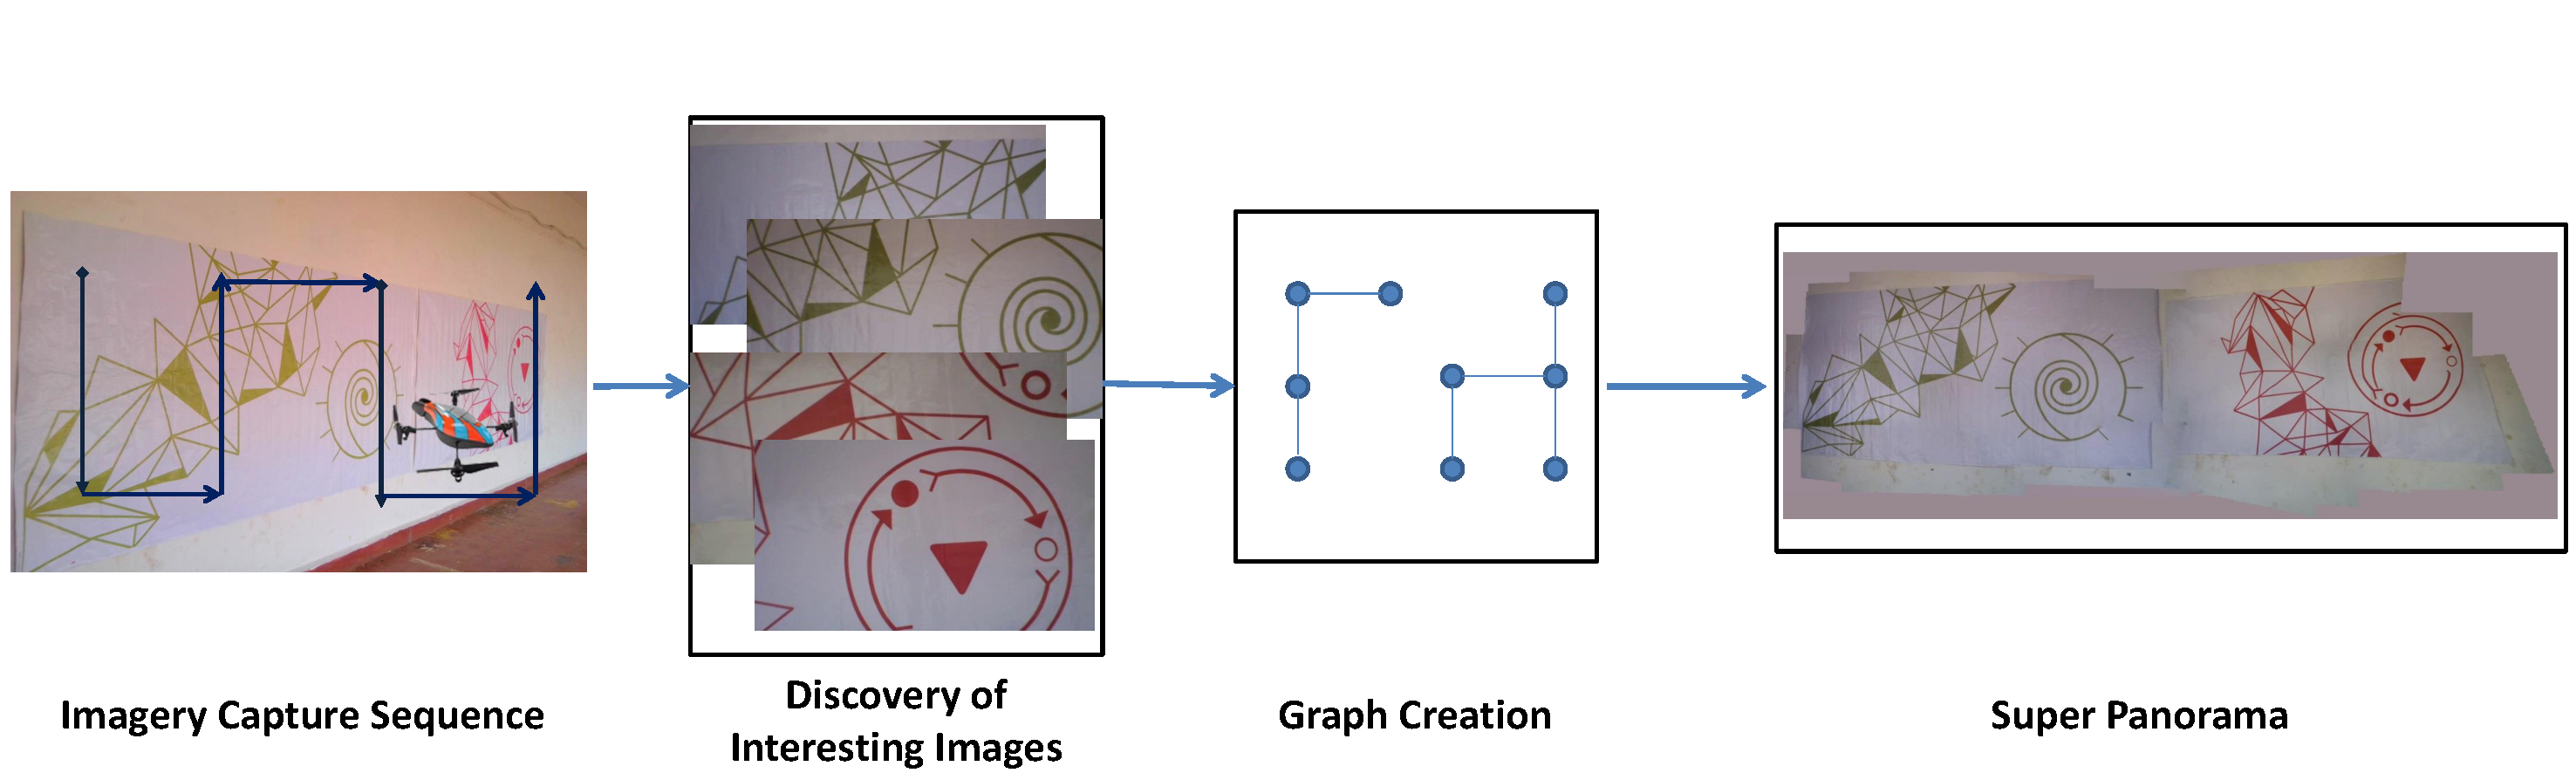
\includegraphics[width=0.49\textwidth]{figures/Workflow} 
  \caption{ \label{fig:workflow} Overview: Input imagery is
    systematically acquired (top Row, column 1) by a quadcopter.  In the next
    step (top row, column 2), interesting images are found by clustering
    the video into regions based on IMU data.  A graph (top row, column 3) is
    constructed by finding homography among only neighbourhood(
    established from again IMU data) images. For each connected component in a
    graph, a mini-panoramas is created (bottom row, right column) which are then
    joined together into super panorama (bottom row, left column)using IMU
    data.}
\end{figure}    


\subsection{Video acquisition}
We first despatch the quadcopter to as close to the scene as
possible. The corners of a rectangular area of interest is provided to
the quadcopter, and it is programmed to traverse the area in a snake
like raster scan fashion.  There are various control aspects involved
in sending a quadcopter; in outdoor areas, the quadcopter is impacted
by wind and it might lose its way.  The control aspects of the
quadcopter is beyond the scope of this paper.

The quadcopter returns with a video of the scene.  Any short video of
about a minute or more when given to a stitching program such as
Autostitch overwhelms the programs rendering it unusable. In the rest
of this section, we use Autostitch to indicate state of the art
stitching programs such as Autostitch, Photoshop, etc.

\subsection{Acquiring interesting images}
Our goal in this step is to reduce the amount of input data and produce a
set of interesting images.  In other words, we wish to convert a video
into an album of images.  We employ fairly standard methods available
in the literature.  For each frame, we compute a set of global image
descriptors such as color histogram, edges, and so on, and run a
clustering algorithm.  The number of cluster centers is generally
determined by the deemed capacity of, say, Autostitch.

The key difference between our problem and standard albumization is
the use of approximate positional information.  A standard quadcopter
has an Inertial Measurement Unit (IMU) that, after calibration, can
give  approximate information of positions.  It is to be noted that
this information can be quite incorrect.  However the mix of
positional information and image features is often sufficient to
produce the necessary subset of `interesting images' which may now
be given as input to Autostitch. Figure~\ref{fig:selection} shows this
process. 

\begin{figure}[h!]
  \centering
  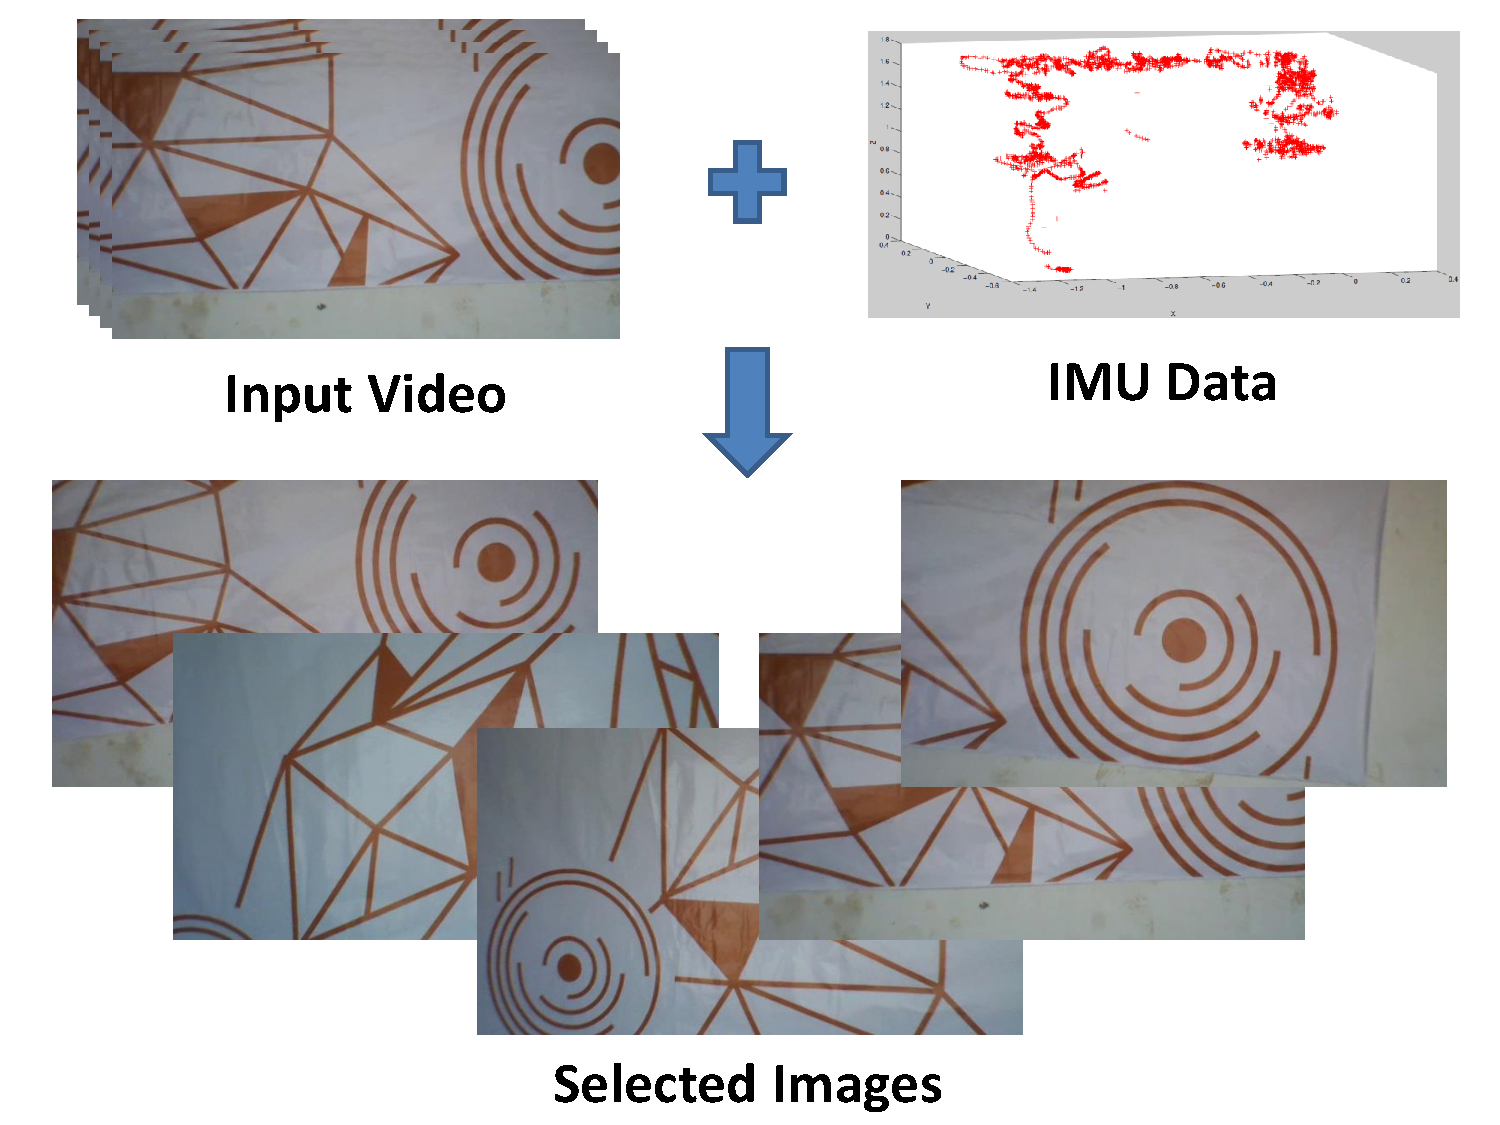
\includegraphics[width=0.49\textwidth]{figures/selection} 
  \caption{ \label{fig:selection}  Using IMU data, an image stream is
  transformed into a set of interesting images for purposes of panorama creation. IMU
    data is hierarchically clustered to find out positions which may cover the
    imaging space. Clustering threshold is kept in a such a way that images
    taken from these points will cover whole scene optimally.}
\end{figure}    


As mentioned in the introduction, as long as there are sufficiently
varying and ``matchable'' features, Autostitch is able to perform a
pleasant stitching.  However, if the features are in the ``wrong''
positions, then the output is not acceptable.

Significantly, Autostitch has not been designed to use positional
information. As a result if there are N input images, the program has
to consider possible matches in an $O(N^2)$ set of areas.  Our program
is able to mosaic in an $O(N)$ fashion.
 
Specifically, we assume at this point that the interesting photos are
available in the form of a $m \times n$ grid. We create a graph with
images being nodes, and postulate edges between two nodes if we are
able to ``do successful matches''. Recall at this point that if there
are ``dead spaces'' there will not be enough features for successful
matches; the graph will end up with multiple (disconnected)
components.  We next compute multiple spanning trees for the various
components. If the result is single tree, then we stitch all pictures
using the homographies.  The spanning tree is an $O(N)$ structure. The
process is described in Figure~\ref{fig:graph}.

\begin{figure}[h!]
  \centering
  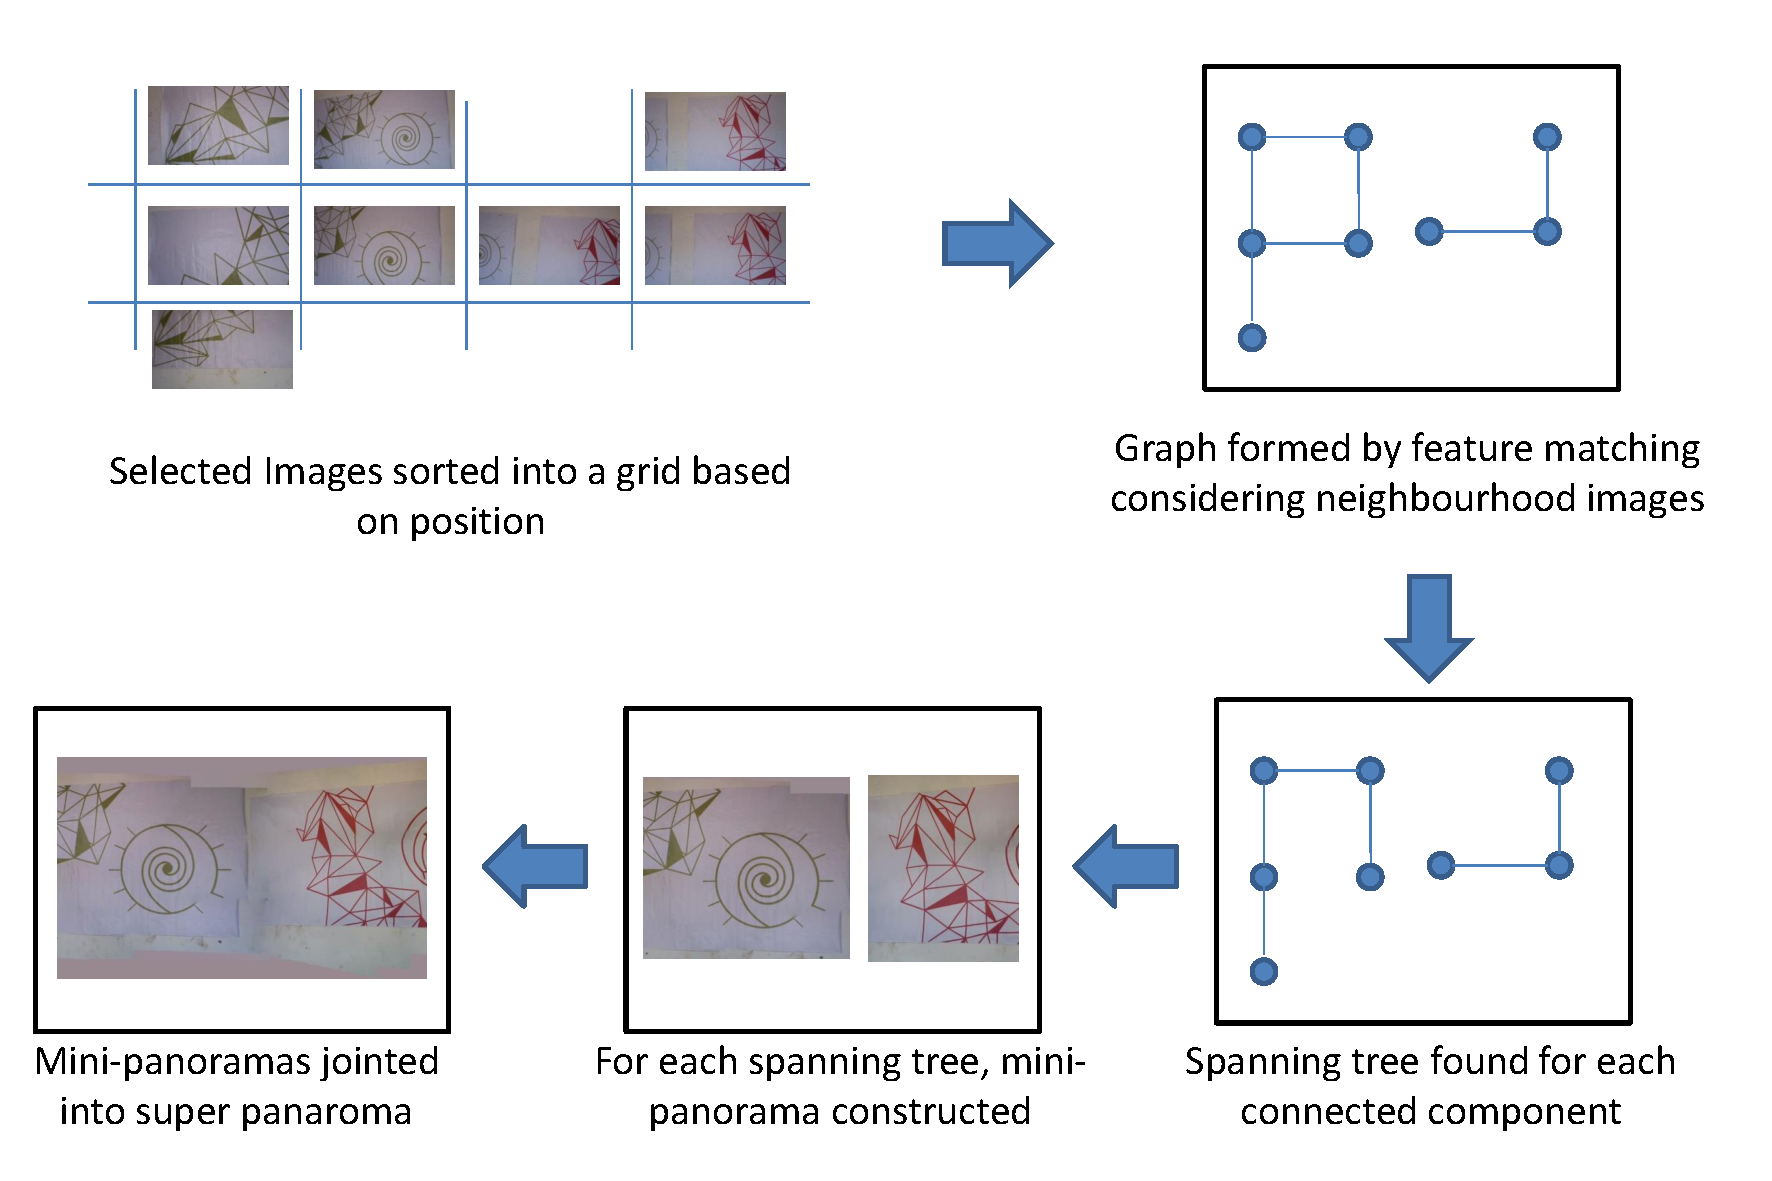
\includegraphics[width=0.49\textwidth]{figures/graph} 
  \caption{ \label{fig:graph} Interesting images acquired are
    segmented and individual (mini-panoramas) are constructed. These
    are then later combined into the desired (super)panorama using IMU data.}
\end{figure}    


\subsection{Super-panoramas}
We assume that the output of the previous step has resulted in
multiple spanning trees where each cluster center corresponds to a
specific depth. We now create individual panoramas for each spanning
tree; we term these as mini-panoramas. We then proceed to create the
desired output, termed super-panorama.  A super-panorama must be
created from mini-panoramas; these usually correspond to different
depths for at least two reasons.

First, it is invariably difficult, if not impossible, to control a
quadcopter to be at the exact depth even in indoor scenes.  The
aerodynamics and the thrust produced tends to make the quadcopter
drift.  Second, it might also be necessary to let the quadcopter probe
and come closer to the scene so as to get a ``good picture''.

A super-panorama is done using a two step process. Assume two trees in
the forest corresponding to area A and area B of the scene (see
Figure~\ref{fig:stereo}). 
\begin{figure}[h!]
  \centering
  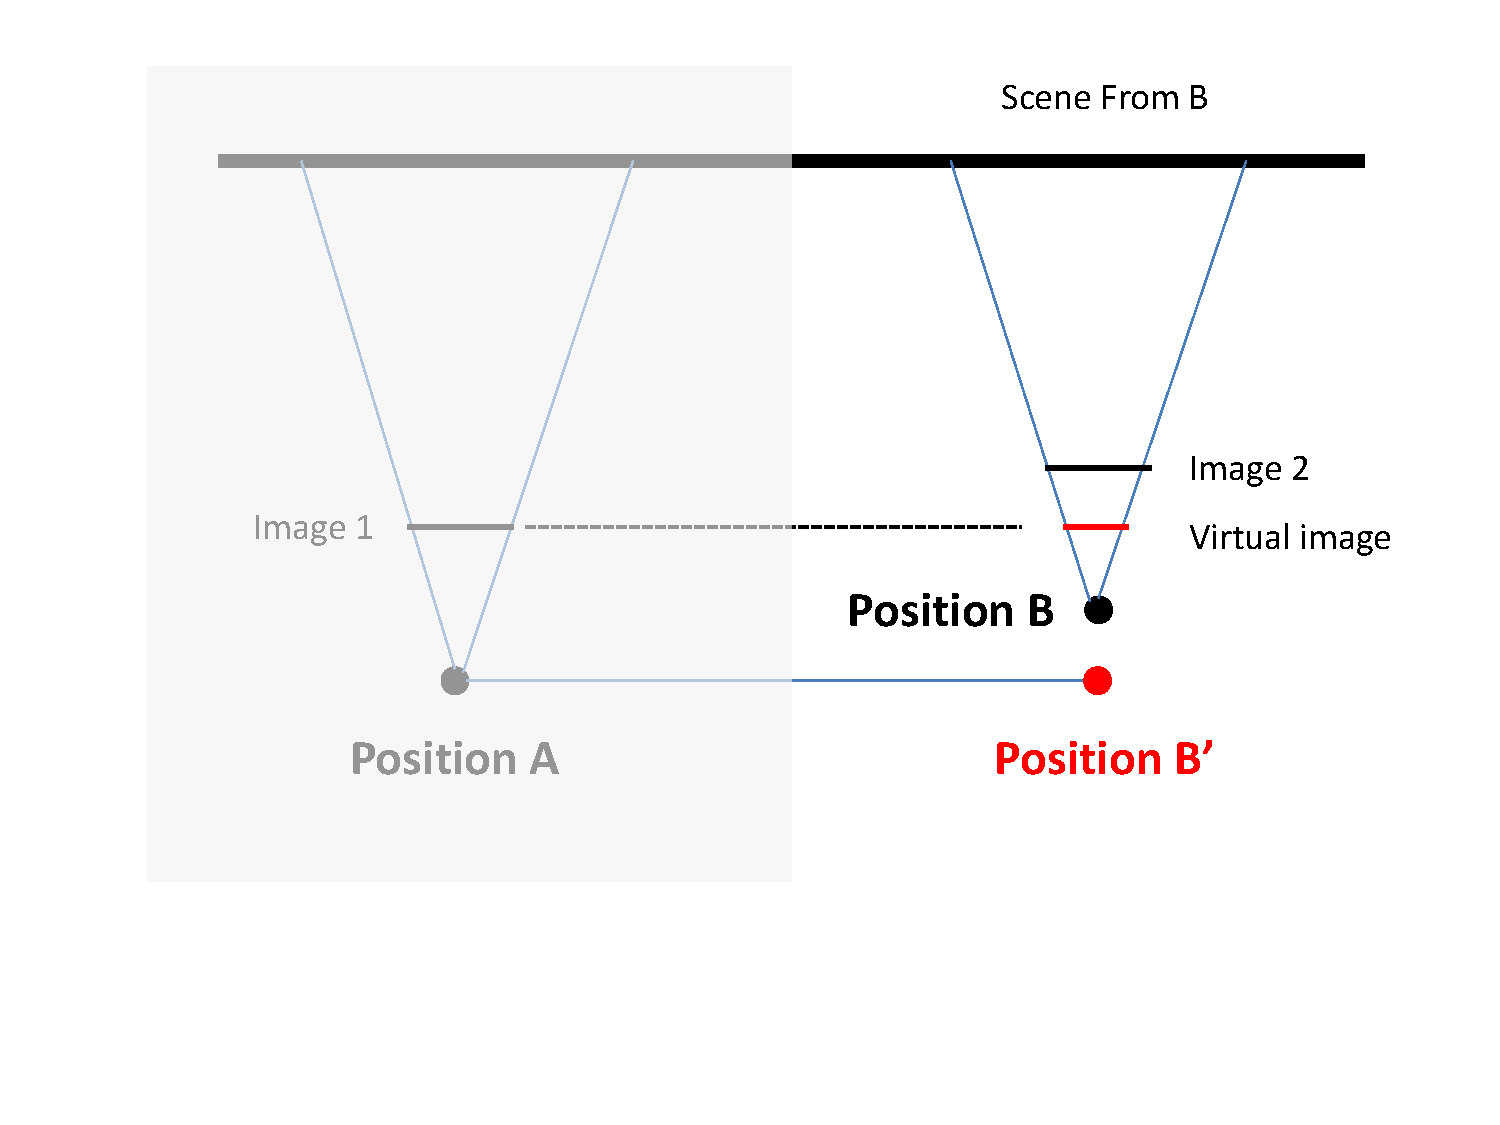
\includegraphics[width=0.4\textwidth]{figures/move} \\
  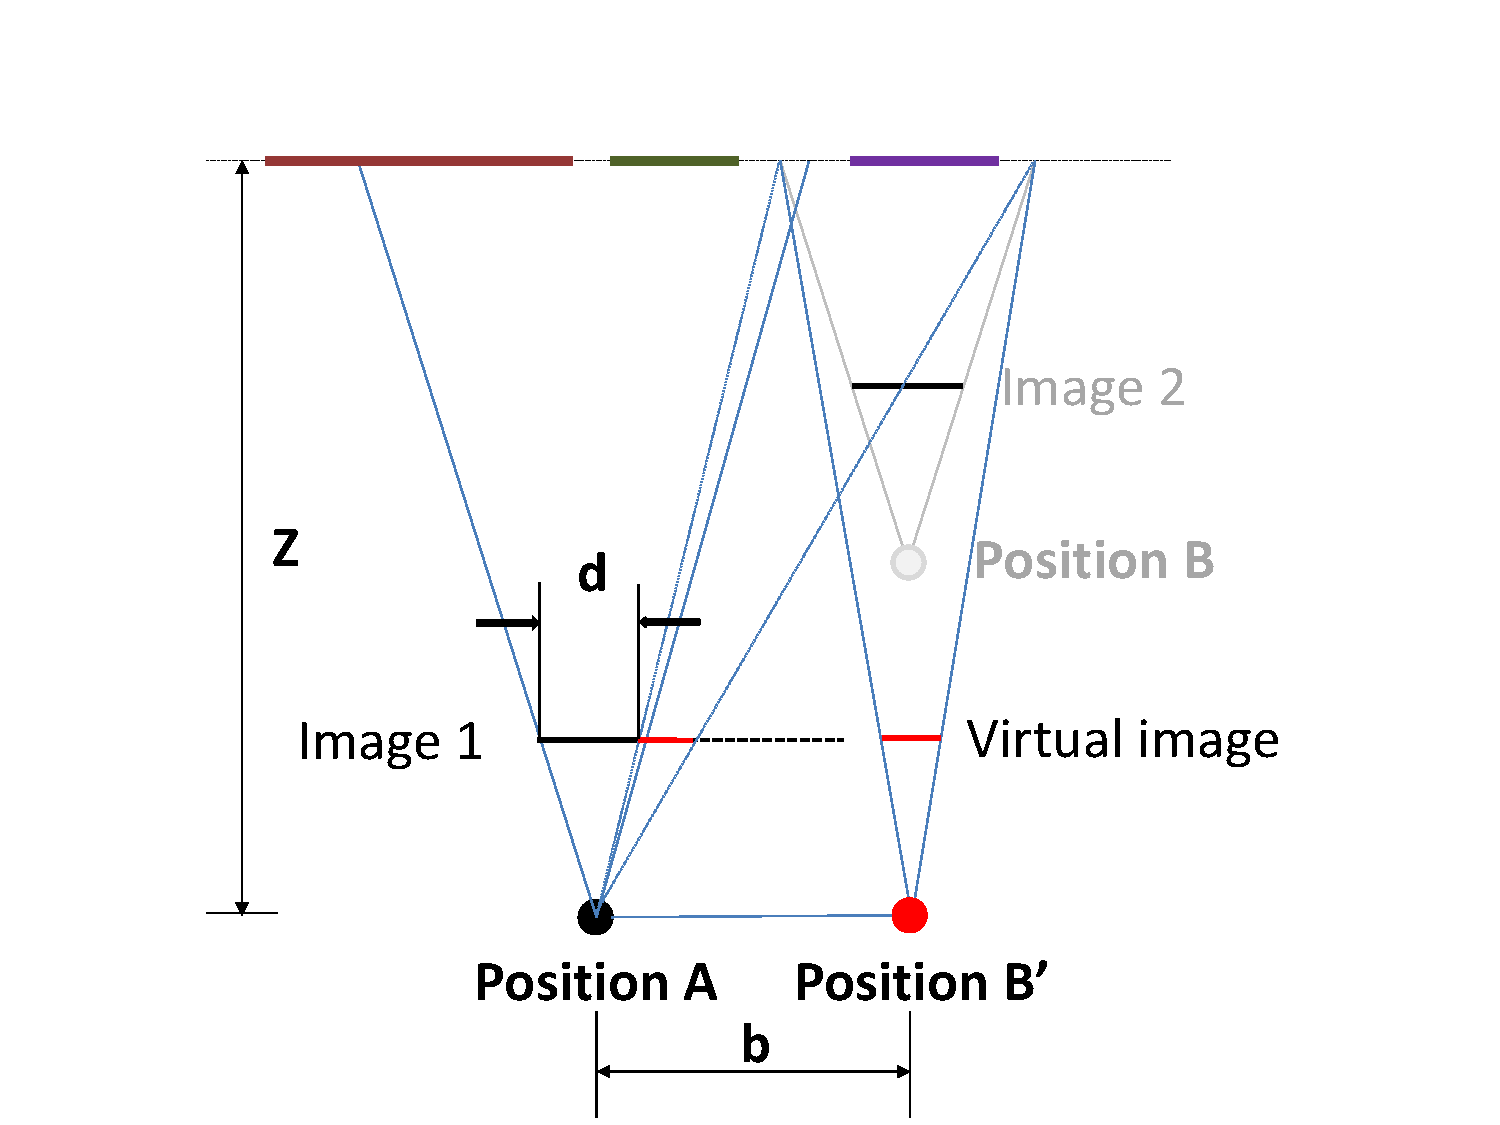
\includegraphics[width=0.4\textwidth]{figures/stereo} 
  \caption{ \label{fig:stereo} Top: The virtual picture as seen from position B'
    is computed using Equation~\ref{eq:moveRelation} from the real picture
    taken from B.  Bottom: Using the disparity, and the baseline width
  it is possible to compute the scene from the view point of A.}
\end{figure}    
Assume that a mini-panorama is created from these two areas, and the
depth of the planar surface from the camera is more for A, than for
B. We then take the mini-panorama image captured at B, and `move' it to
a new location B’ whose depth (from the imaged wall) is the same as
that of A. The resulting image  will be smaller than: the images are
related by the equation
\begin{equation}
  \label{eq:moveRelation}
  {\bf \frac{x'}{x} = \frac{Z}{Z'}}
\end{equation}

We can now treat the resulting images from A (unchanged) and B’
(computed from Equation~\ref{eq:moveRelation}) forming a stereo pair.
Using the stereo disparity formula we can ``place'' the image from B from the
view point of A thereby creating a super-panorama.

\section{Experiments and Results}
\label{sec:results}

All our experiments have been completed with the inexpensive consumer
quadcopter called Parrot's AR Drone 2.0. We have used the ROS based
ARDrone Autonomy Driver to communicate with the drone. For the
purposes of establishing the ground truth, pictures were taken with a
5 mega pixel camera.

We have implemented our algorithm in C++ using the OpenCV library
(OpenCV 2.4.9). Experiments were performed on a PC with Intel Core i7
processor(@3.4GHz) and 8GB RAM.  The source code to produce
interesting images from a video, and to generate the super-panorama,
as well as the data sets used in this paper will be made publicly
available.


\subsection{Establishing Correctness}

In our first experiment, we wanted to ensure that the selection of
images done was comprehensive.  We sent the drone to recce an outdoor
scene with no dead space. This experiment was conducted in an outdoor
environment. We note here that there were approximately 9000 images in
the raw video.  Autostitch was unable to cope when fed with this large
number. 

One way to produce some sort of mosaic was to simply reduce the amount
of data given to Autostitch.  Figure \ref{fig:uniformsampled_sac3}
shows uniformly time sampled images from complete video.  When these
uniformly sampled images are given to Autostitch or to Adobe
Photoshop, we find (Figure \ref{fig:results_sac3_timesmapled})  that the
results are not satisfactory.

Instead of feeding time-sampled images, we ran our saliency selection
algorithm on the video. Figure \ref{fig:selected_sac3} shows examples of
selected images. Many of the images are similar to the time sampled
version; however, the occasional differences are enough to make
Autostitch work. 

Using only $N=5$ images, the results are shown in
Figure~\ref{fig:results_sac3_timesmapled}.


\begin{figure*}[htb!]
\centering

\includegraphics[width=0.19\linewidth]{figures/sac3/uniform_sampled/1.jpg}
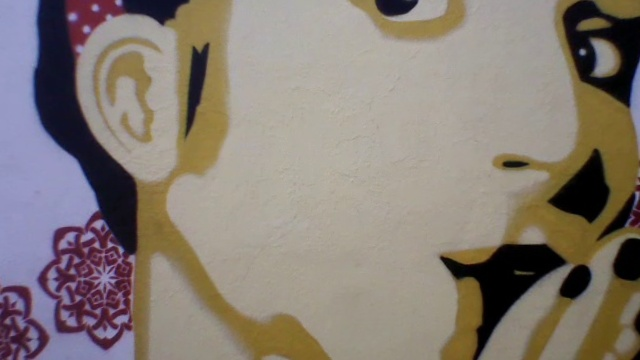
\includegraphics[width=0.19\linewidth]{figures/sac3/uniform_sampled/5.jpg}
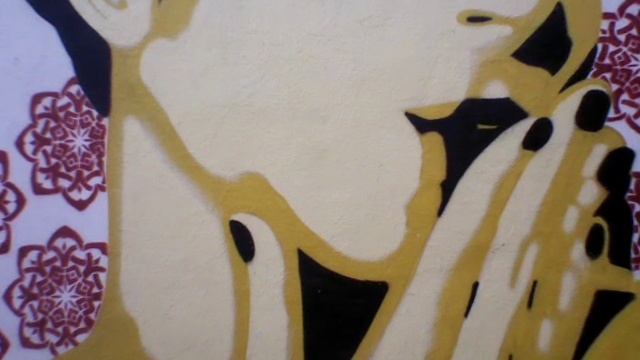
\includegraphics[width=0.19\linewidth]{figures/sac3/uniform_sampled/4.jpg}
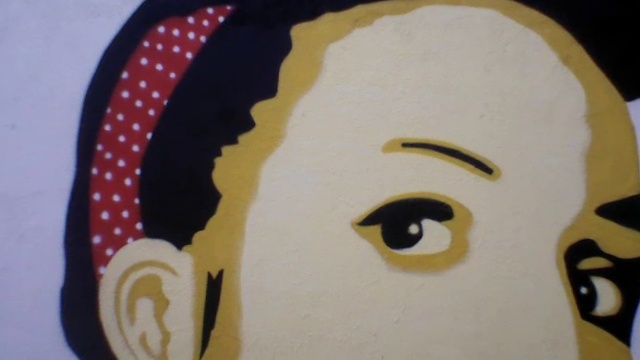
\includegraphics[width=0.19\linewidth]{figures/sac3/uniform_sampled/2.jpg}

\includegraphics[width=0.19\linewidth]{figures/sac3/uniform_sampled/3.jpg}
\caption{Uniformly sampled images from an outdoor video expedition.}
\label{fig:uniformsampled_sac3}
\end{figure*}

\begin{figure*}[t!]
\centering
\begin{subfigure}[b]{0.4\textwidth}
\centering
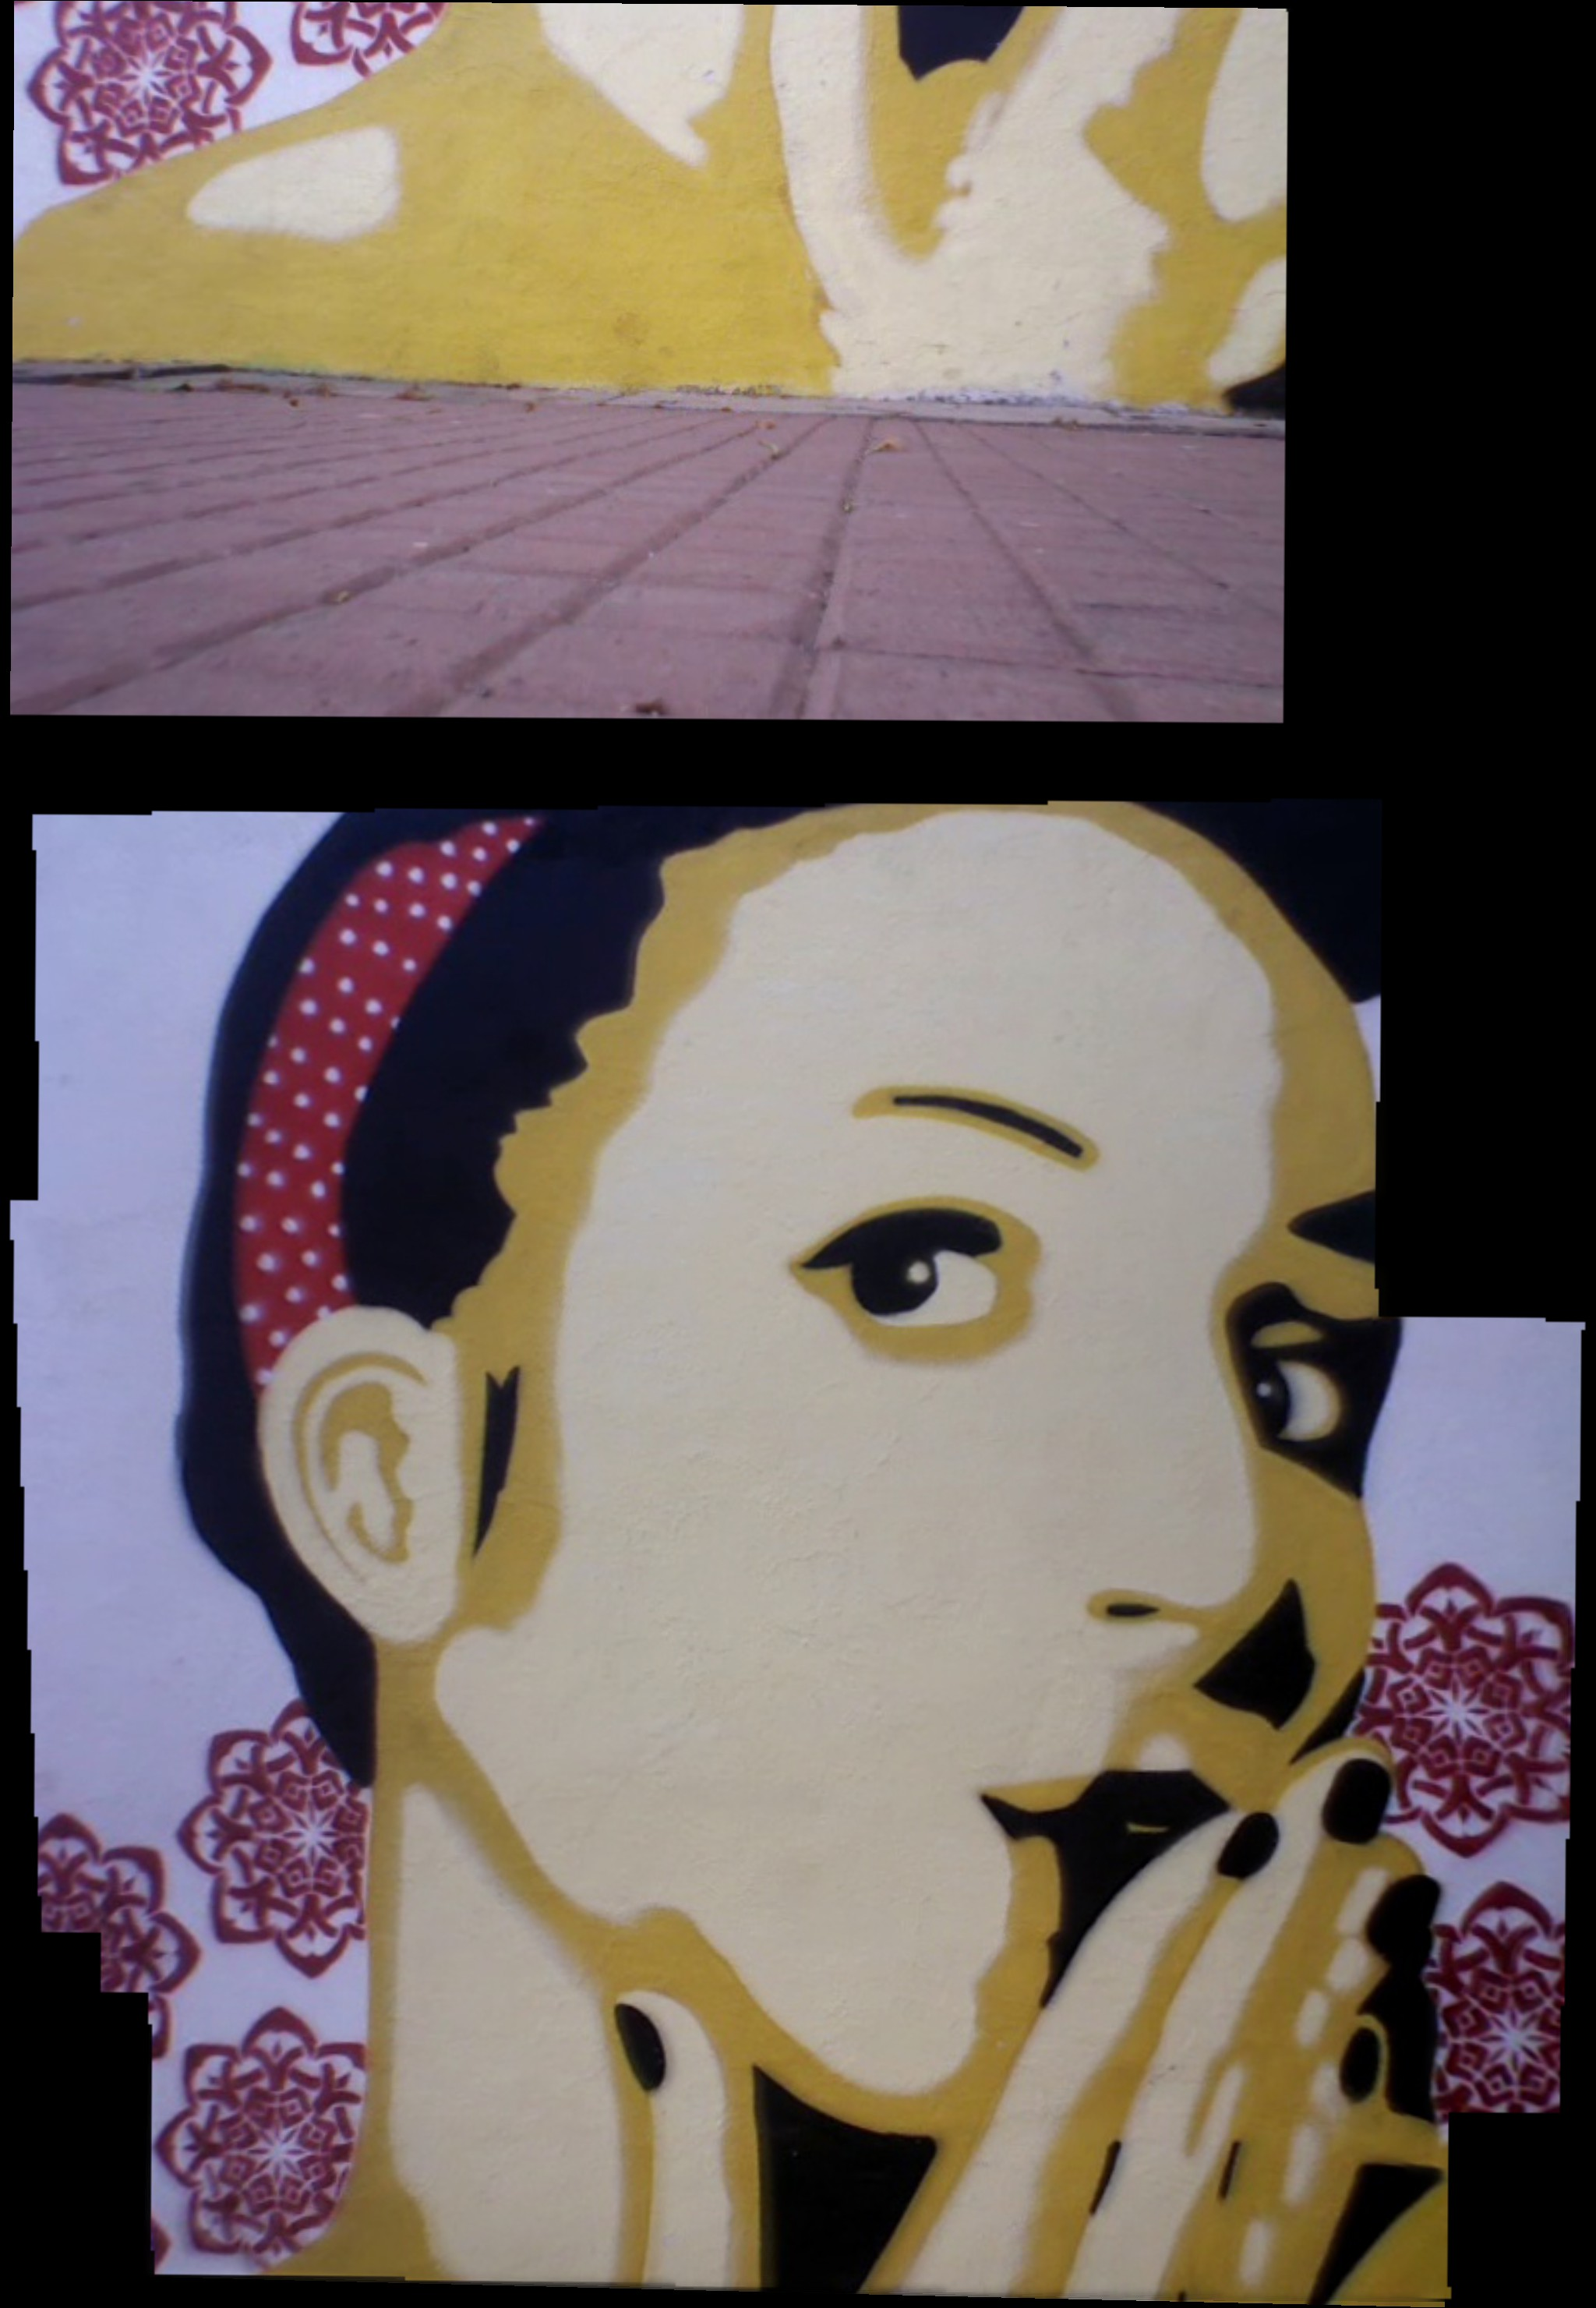
\includegraphics[width=\linewidth]{figures/sac3/uniform_sampled/autostitch.jpg}
\caption{Autostitch Result}
\end{subfigure}
\begin{subfigure}[b]{0.4\textwidth}
\centering
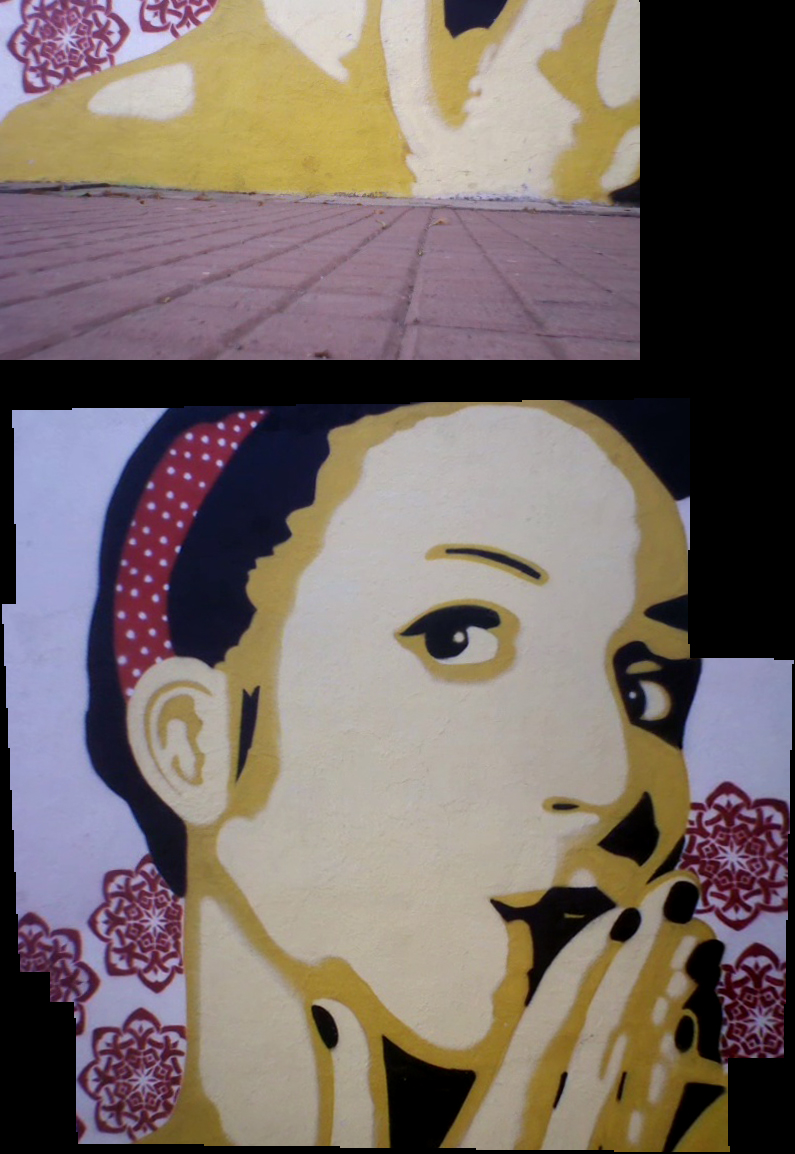
\includegraphics[width=\linewidth]{figures/sac3/uniform_sampled/photoshop.jpg}
\caption{Photoshop Result}
\end{subfigure}
\caption{Output of state of the art photo stitchers on uniformly time
  sampled images. As time sampled images do not guarantee 
  coverage of the scene, the panorama is broken. The top portions do
  not belong at the right place (see Figure~\ref{fig:results_sac3})}
\label{fig:results_sac3_timesmapled}
\end{figure*}


\begin{figure*}[htb!]
\centering

\includegraphics[width=0.19\linewidth]{figures/sac3/selected/1.jpg}
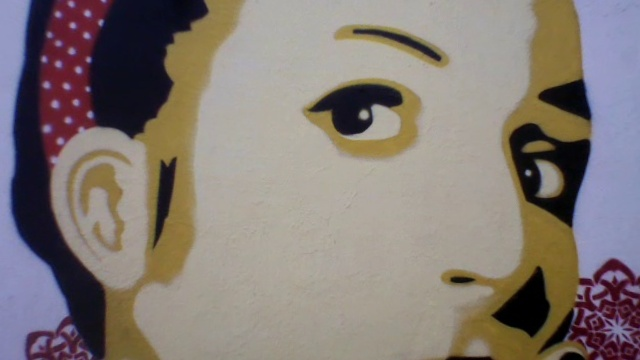
\includegraphics[width=0.19\linewidth]{figures/sac3/selected/5.jpg}
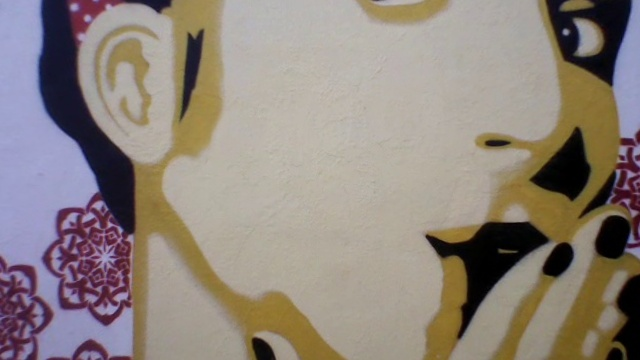
\includegraphics[width=0.19\linewidth]{figures/sac3/selected/4.jpg}
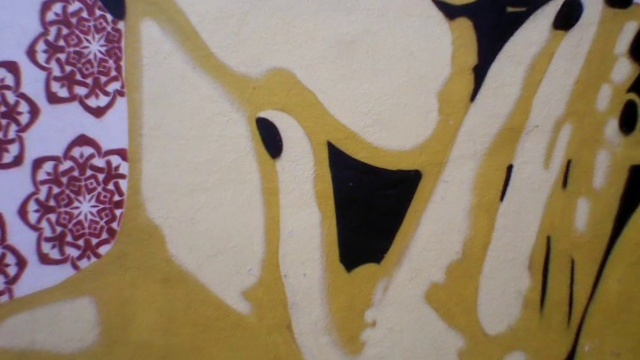
\includegraphics[width=0.19\linewidth]{figures/sac3/selected/2.jpg}

\includegraphics[width=0.19\linewidth]{figures/sac3/selected/3.jpg}
\caption{Salient image selection from the set of approximately 9000
  images using positional information.}
\label{fig:selected_sac3}
\end{figure*}


\begin{figure*}
\centering
\begin{subfigure}[b]{0.3\textwidth}
\centering
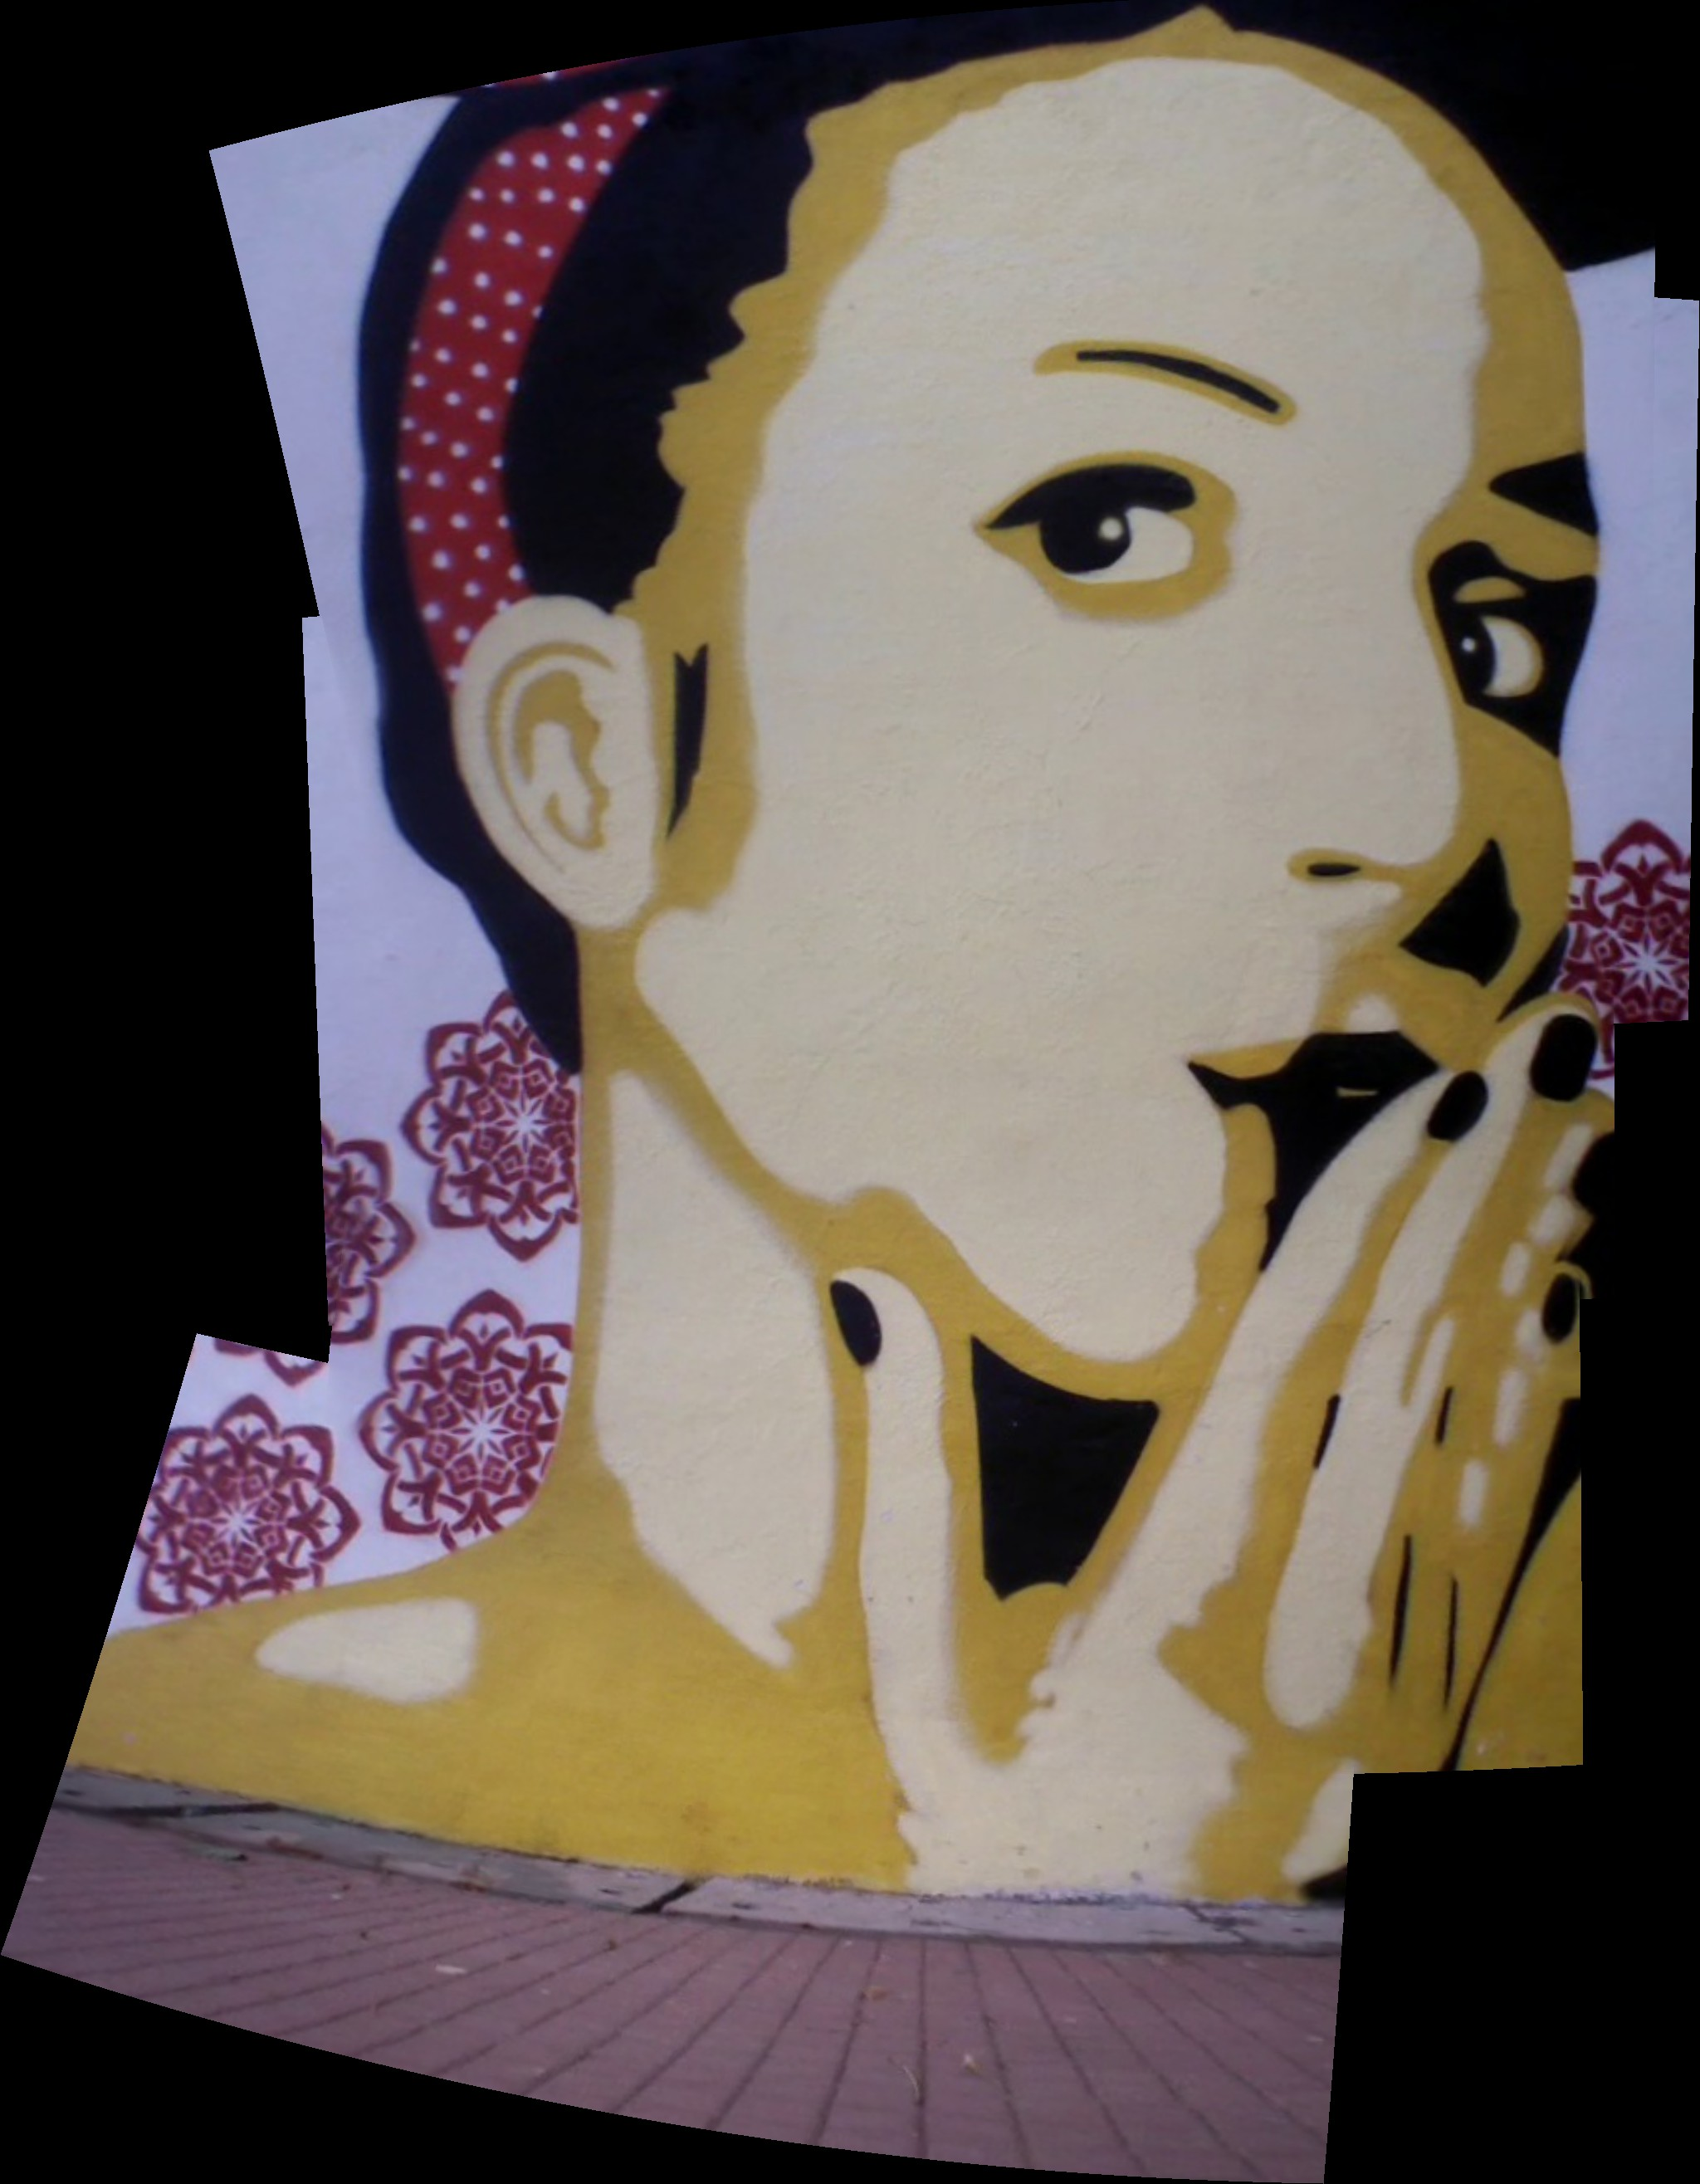
\includegraphics[width=\linewidth]{figures/sac3/autostitch.jpg}
\caption{Autostitch Result}
\end{subfigure}
\begin{subfigure}[b]{0.3\textwidth}
\centering
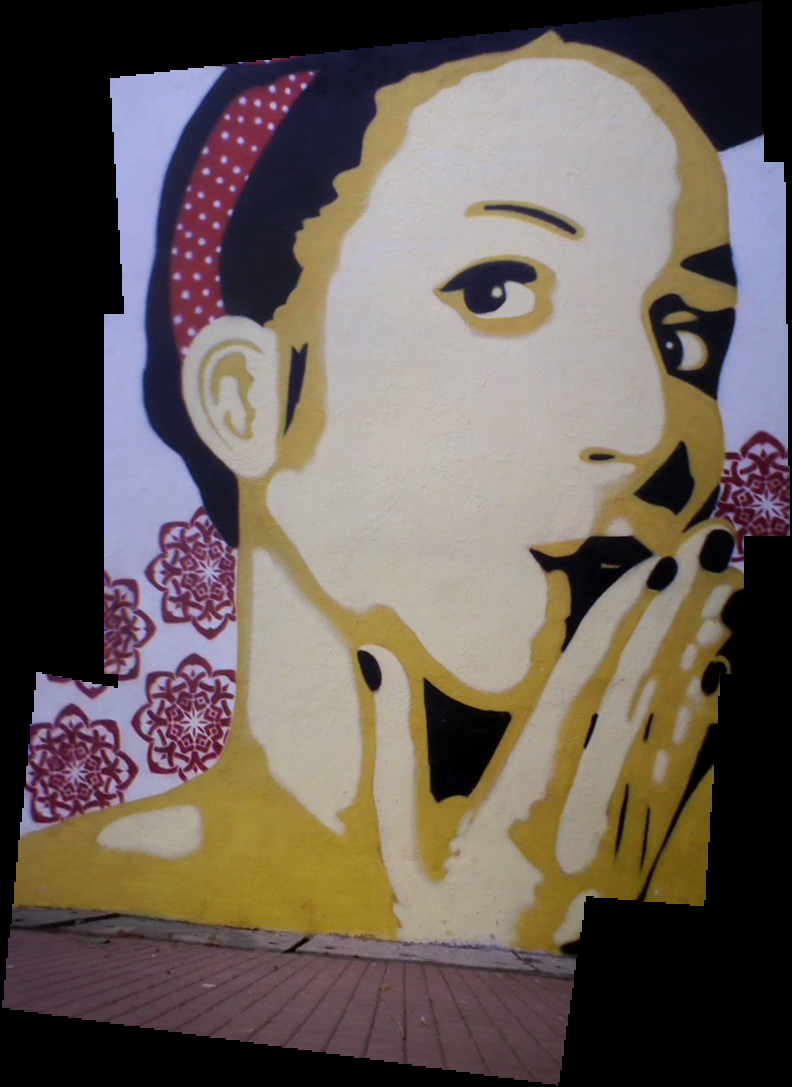
\includegraphics[width=\linewidth]{figures/sac3/photoshop.jpg}
\caption{Photoshop Result}
\end{subfigure}
\begin{subfigure}[b]{0.3\textwidth}
\centering
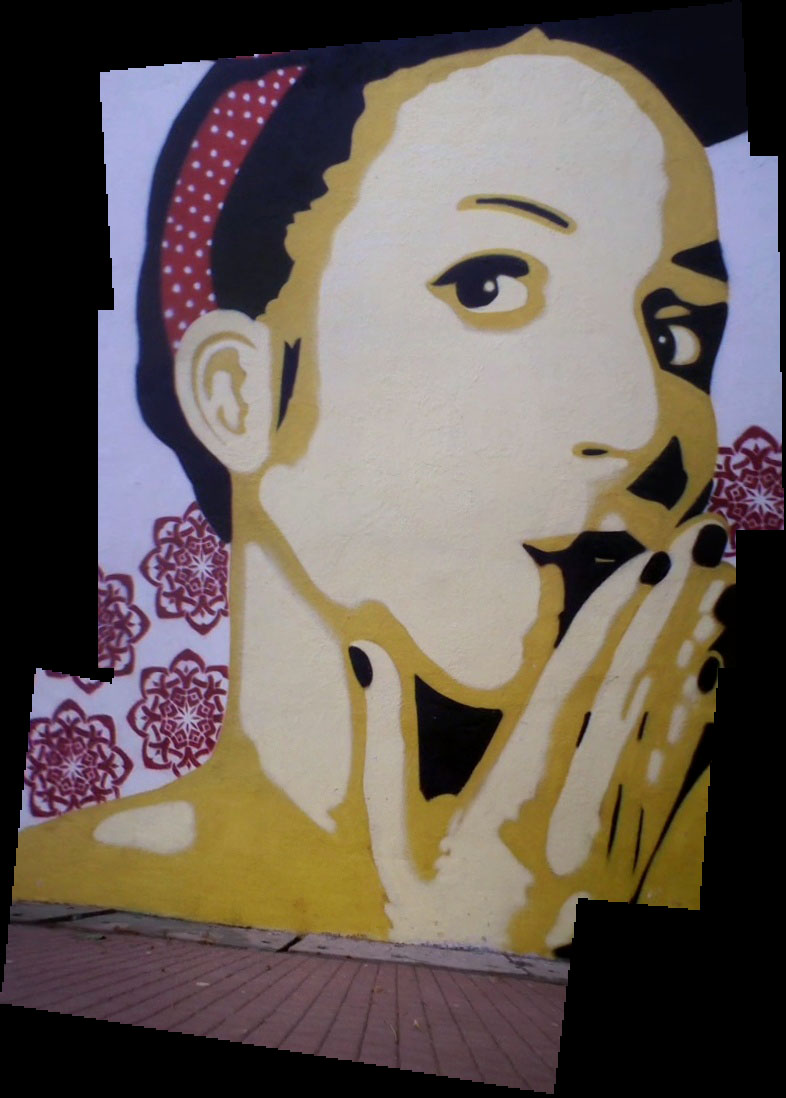
\includegraphics[width=\linewidth]{figures/sac3/our_result.jpg}
\caption{Our Result}
\end{subfigure}
\caption{When salient images are given to Autostich and Photoshop, a
  video can be used to create a panaromic mosaic provided there is no
  dead space. We also show the results from our stitching algorithm.}
\label{fig:results_sac3}
\end{figure*}

In summary, this experiment provides evidence to show that (a) our
saliency selection algorithm is reasonable and (b) our stitching
results are comparable to that of Autostitch for the kind of scenes
considered.

\subsection{Indoor Imagery with Dead Space} 

Our next selection of experiments were conducted in an indoor
environment with some natural light.  The input stream had about 4300
images. The selection algorithm pruned the video into N=4 images. A
sample of the selected images are seen in Figure~\ref{fig:idc_selected}

\begin{figure}
\centering

\includegraphics[width=0.22\linewidth]{figures/idc_indoor/selected/1.jpg}
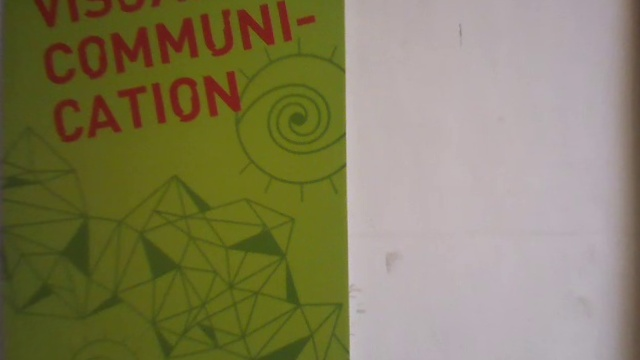
\includegraphics[width=0.22\linewidth]{figures/idc_indoor/selected/2.jpg}

\includegraphics[width=0.22\linewidth]{figures/idc_indoor/selected/3.jpg}

\includegraphics[width=0.22\linewidth]{figures/idc_indoor/selected/4.jpg}
\caption{Pruned images from a video of an indoor scene.}
\label{fig:idc_selected}
\end{figure}

There were two disconnected components in the resulting graph.
Autostitch was unable to produce any reasonable output as seen in
Figure~\ref{fig:idc_indoor_comparison}.  The ground truth can be seen
in Figure~\ref{fig:idc_indoor_groundtruth}.  One can see a better
orthographic view of the posters in a composite manner.


\begin{figure}[p]

\includegraphics[width=\linewidth]{figures/idc_indoor/groundtruth.jpg}
\caption{Ground truth of the indoor scene.  There is a substantial gap
  in between the two posters, and this dead space confuses state of the
  art stitchers since they do not find features.}
\label{fig:idc_indoor_groundtruth}
\end{figure} 

Figure \ref{fig:idc_indoor_comparison} shows the comparison of outputs of state
of the art stitchers with output of our algorithm. 

\begin{figure*}
\begin{subfigure}[b]{0.45\textwidth}

\includegraphics[width=\linewidth]{figures/idc_indoor/autostitch.jpg}
\caption{Autostitch Result}
\end{subfigure}
\begin{subfigure}[b]{0.45\textwidth}

\includegraphics[width=\linewidth]{figures/idc_indoor/photoshop.jpg}
\caption{Photoshop Result}
\end{subfigure}
\begin{subfigure}[b]{\textwidth}

\includegraphics[width=\linewidth]{figures/idc_indoor/our_result.jpg}
\caption{Our Result}
\end{subfigure}
\caption{Comparison of outputs of Autostich, Photoshop and our stitching
algorithm on an indoor scene. Only our
algorithm is able to show a complete super-panorama; state-of-the art
stitchers can produce only one mini-panorama.}
\label{fig:idc_indoor_comparison}
\end{figure*}

One can see a better orthographic view of the posters in a composite
manner. Autostitch was unable to produce any reasonable output as seen in
Figure \ref{fig:idc_indoor_comparison}.

\subsection{Outdoor Imagery with Dead Space}
Our next set of experiments were conducted in an outdoor environment. The  
input stream had about 12000 images. The selection algorithm pruned the video
into N=30 images. A sample of the selected images are seen in Figure
\ref{fig:green_red_selected}.

\begin{figure}
\centering

\includegraphics[width=0.19\linewidth]{figures/green_red/selected/1.jpg}
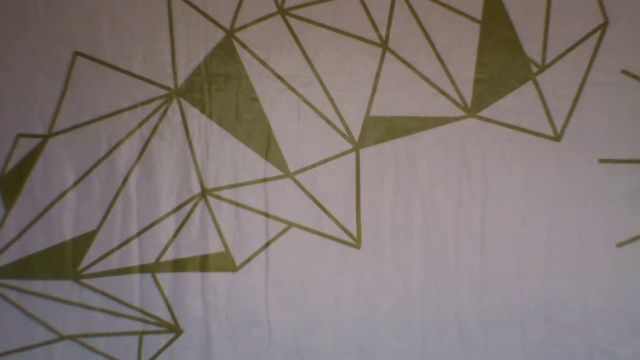
\includegraphics[width=0.19\linewidth]{figures/green_red/selected/2.jpg}

\includegraphics[width=0.19\linewidth]{figures/green_red/selected/3.jpg}
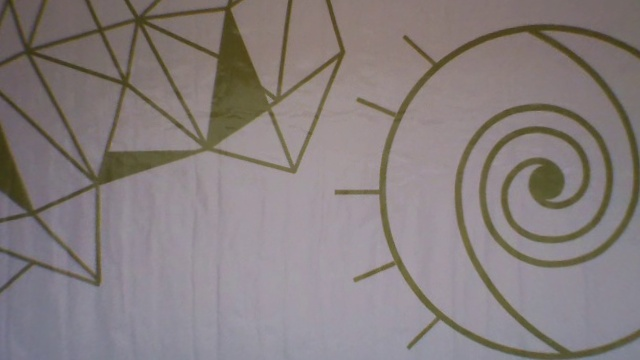
\includegraphics[width=0.19\linewidth]{figures/green_red/selected/4.jpg}
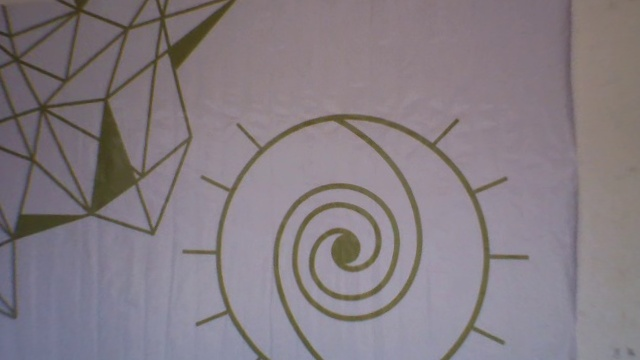
\includegraphics[width=0.19\linewidth]{figures/green_red/selected/5.jpg}
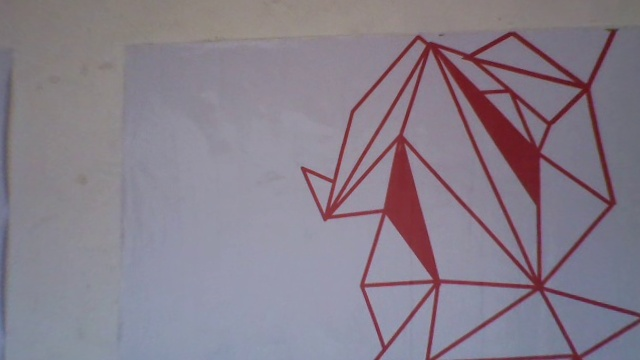
\includegraphics[width=0.19\linewidth]{figures/green_red/selected/6.jpg}
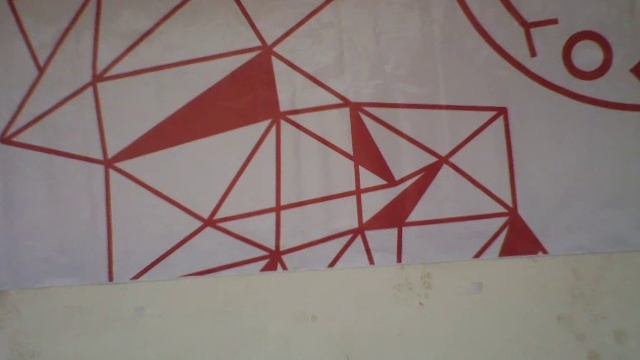
\includegraphics[width=0.19\linewidth]{figures/green_red/selected/7.jpg}
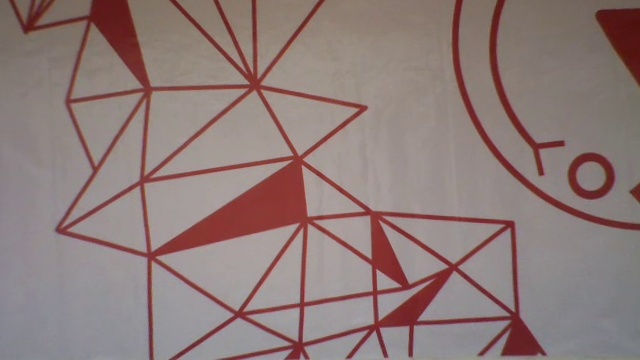
\includegraphics[width=0.19\linewidth]{figures/green_red/selected/8.jpg}
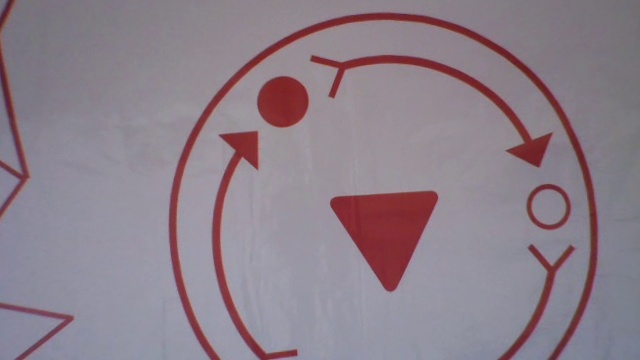
\includegraphics[width=0.19\linewidth]{figures/green_red/selected/9.jpg}
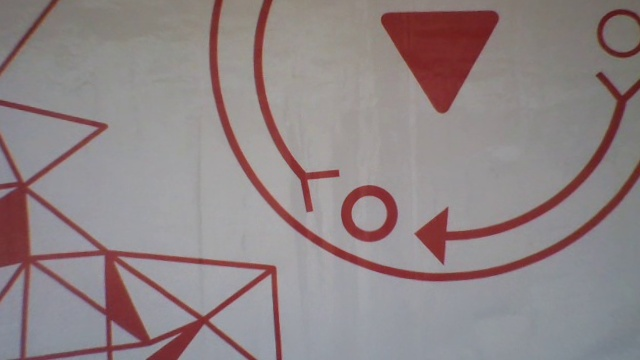
\includegraphics[width=0.19\linewidth]{figures/green_red/selected/10.jpg}
\caption{Sample selected images of outdoor scene by our algorithm.}
\label{fig:green_red_selected}
\end{figure}

The ground truth of outdoor scene can be seen in Figure
\ref{fig:green_red_groundtruth}.

\begin{figure}
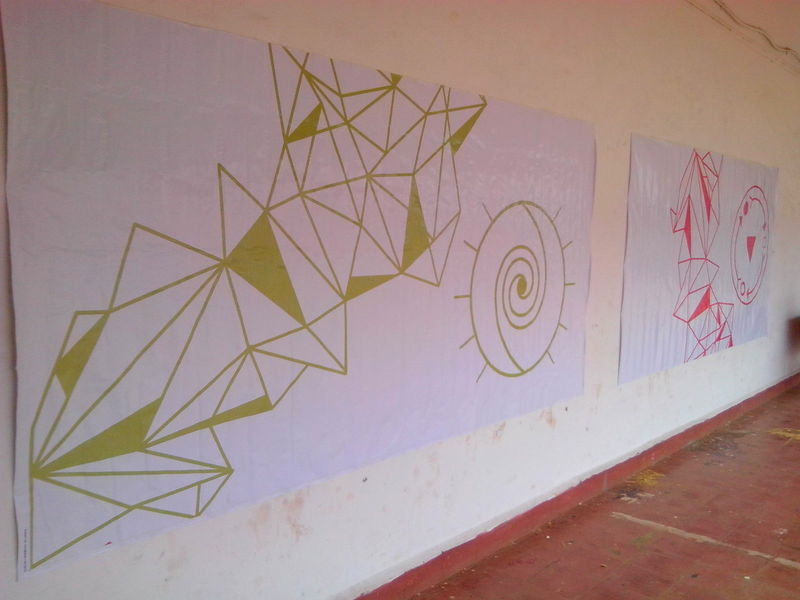
\includegraphics[width=\linewidth]{figures/green_red/groundtruth.jpg}
\caption{Ground truth of the outdoor scene captured by quadcopter. There is
visible gap in between two posters which will cause problems for state of the art
stitchers.}
\label{fig:green_red_groundtruth}
\end{figure}


\begin{figure*}
\begin{subfigure}[b]{0.45\textwidth}
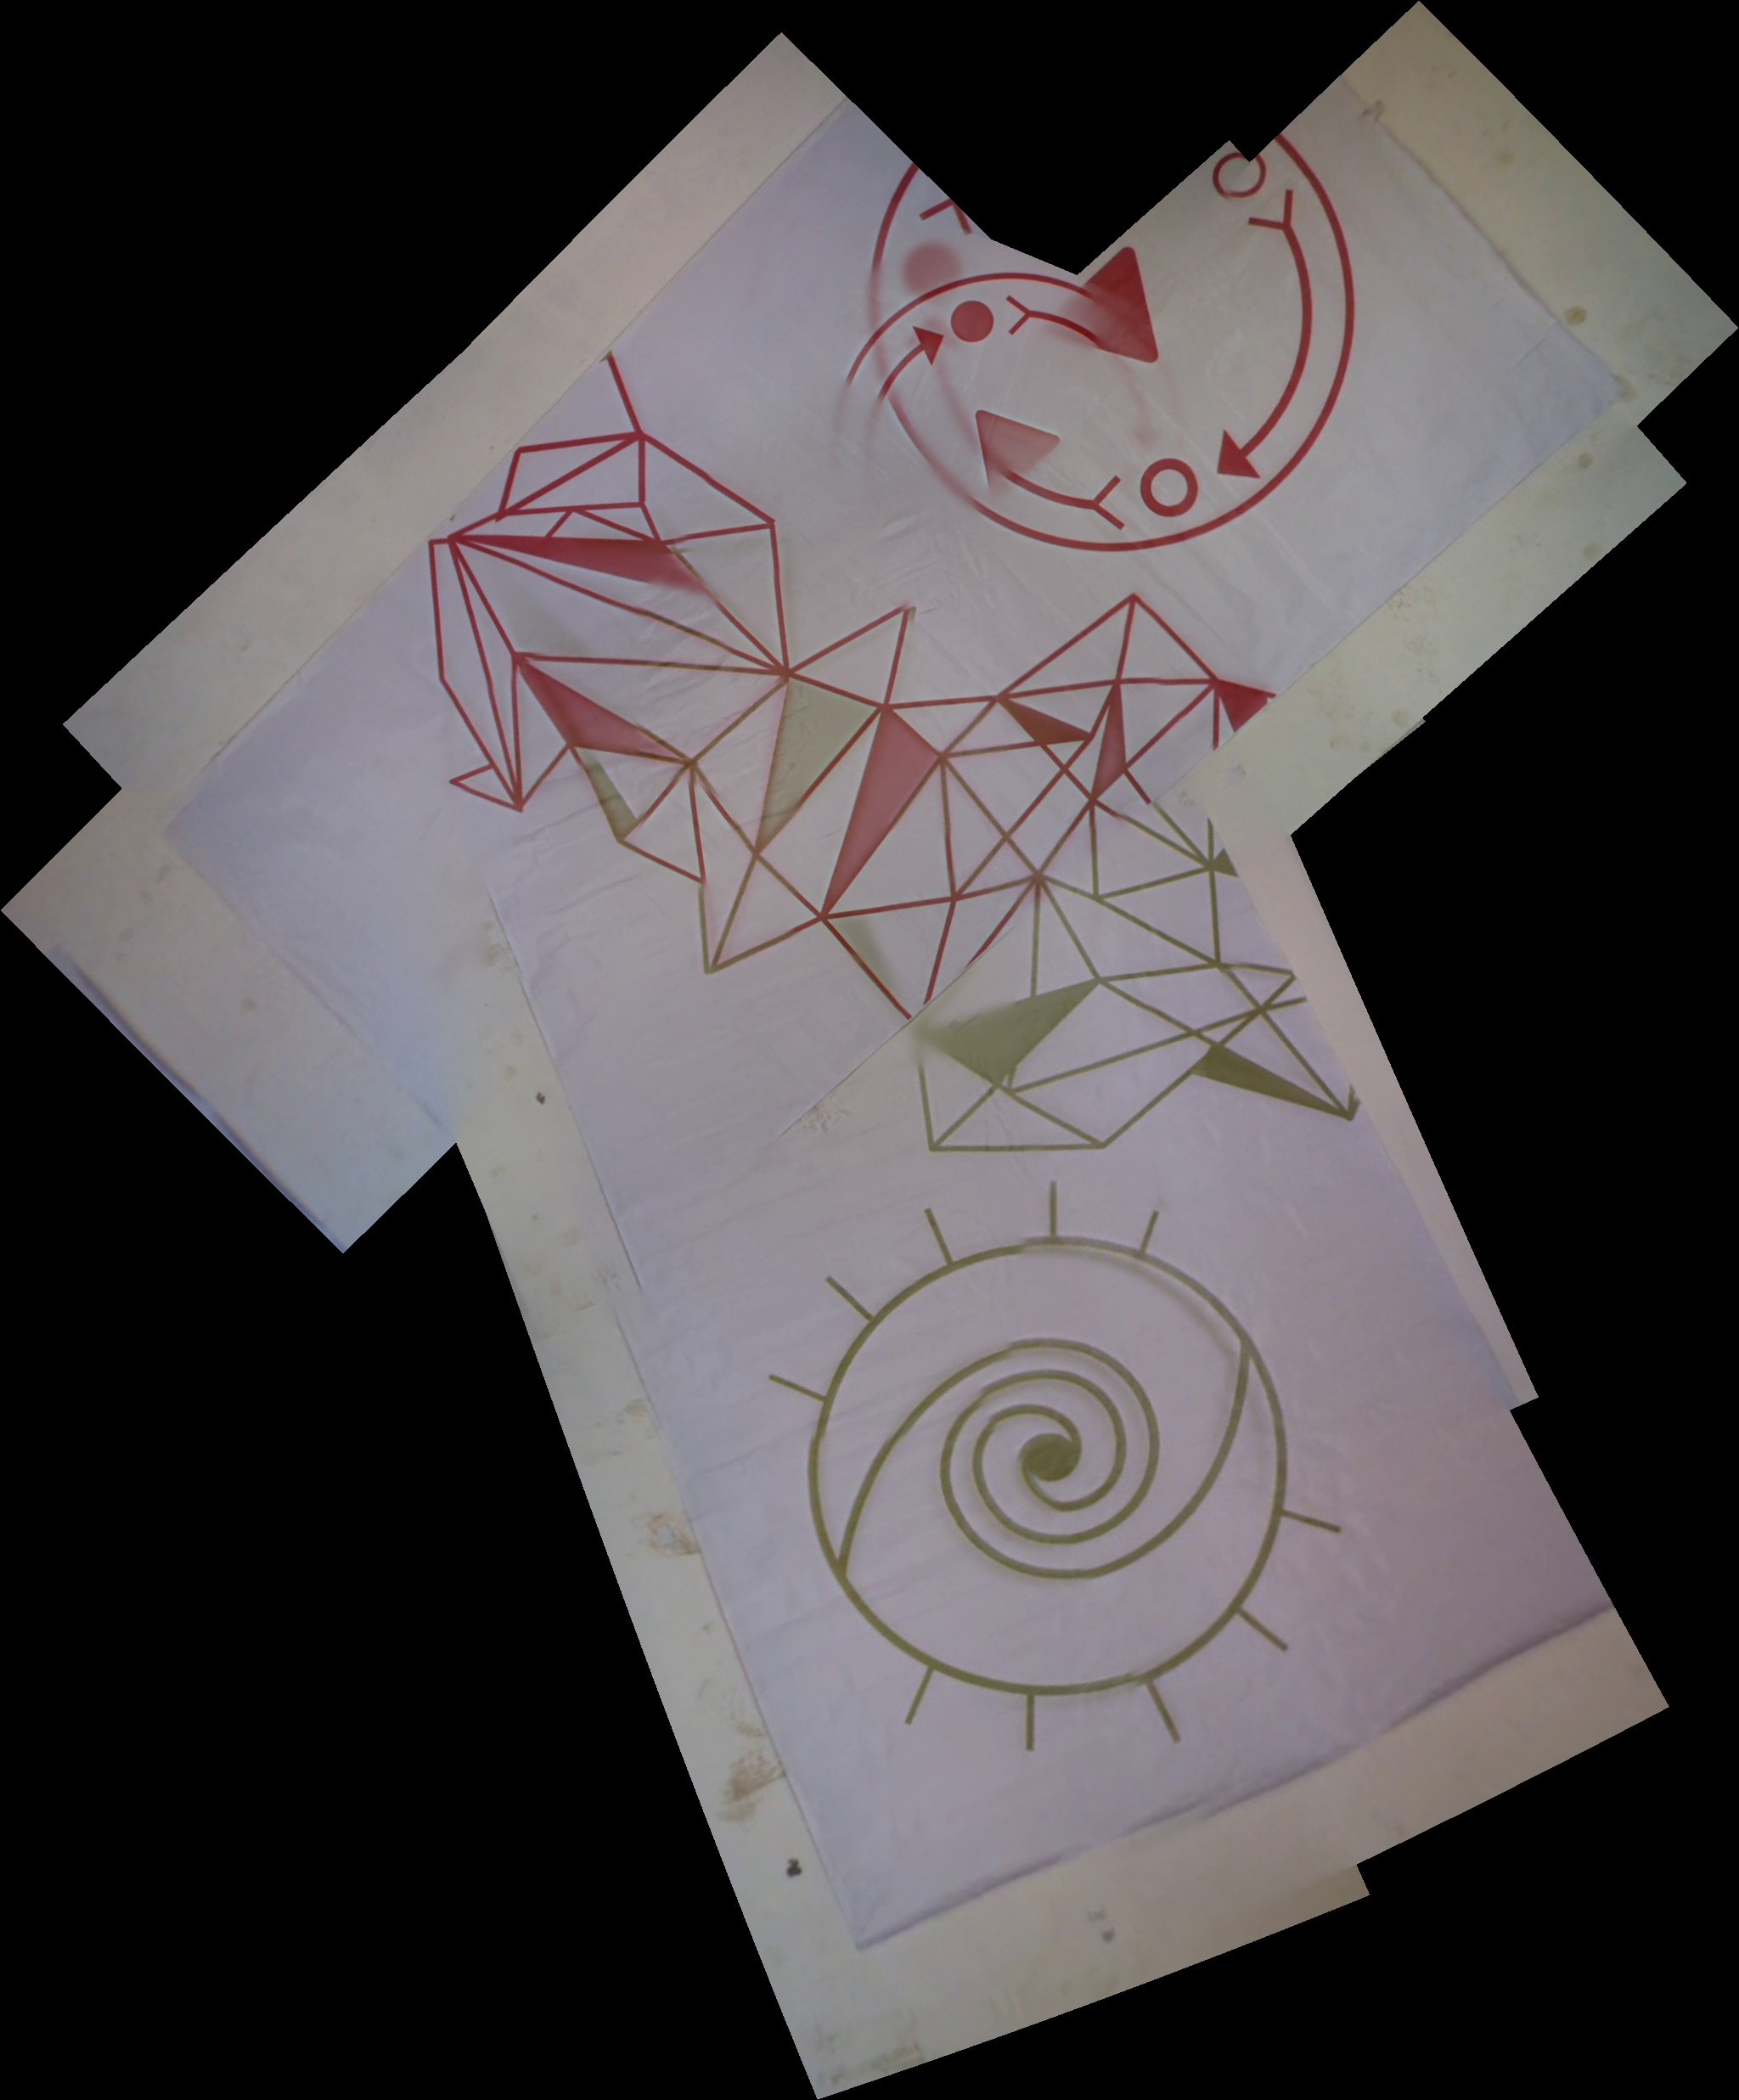
\includegraphics[width=\linewidth]{figures/green_red/autostich.jpg}
\caption{Autostitch Result}
\end{subfigure}
\begin{subfigure}[b]{0.45\textwidth}
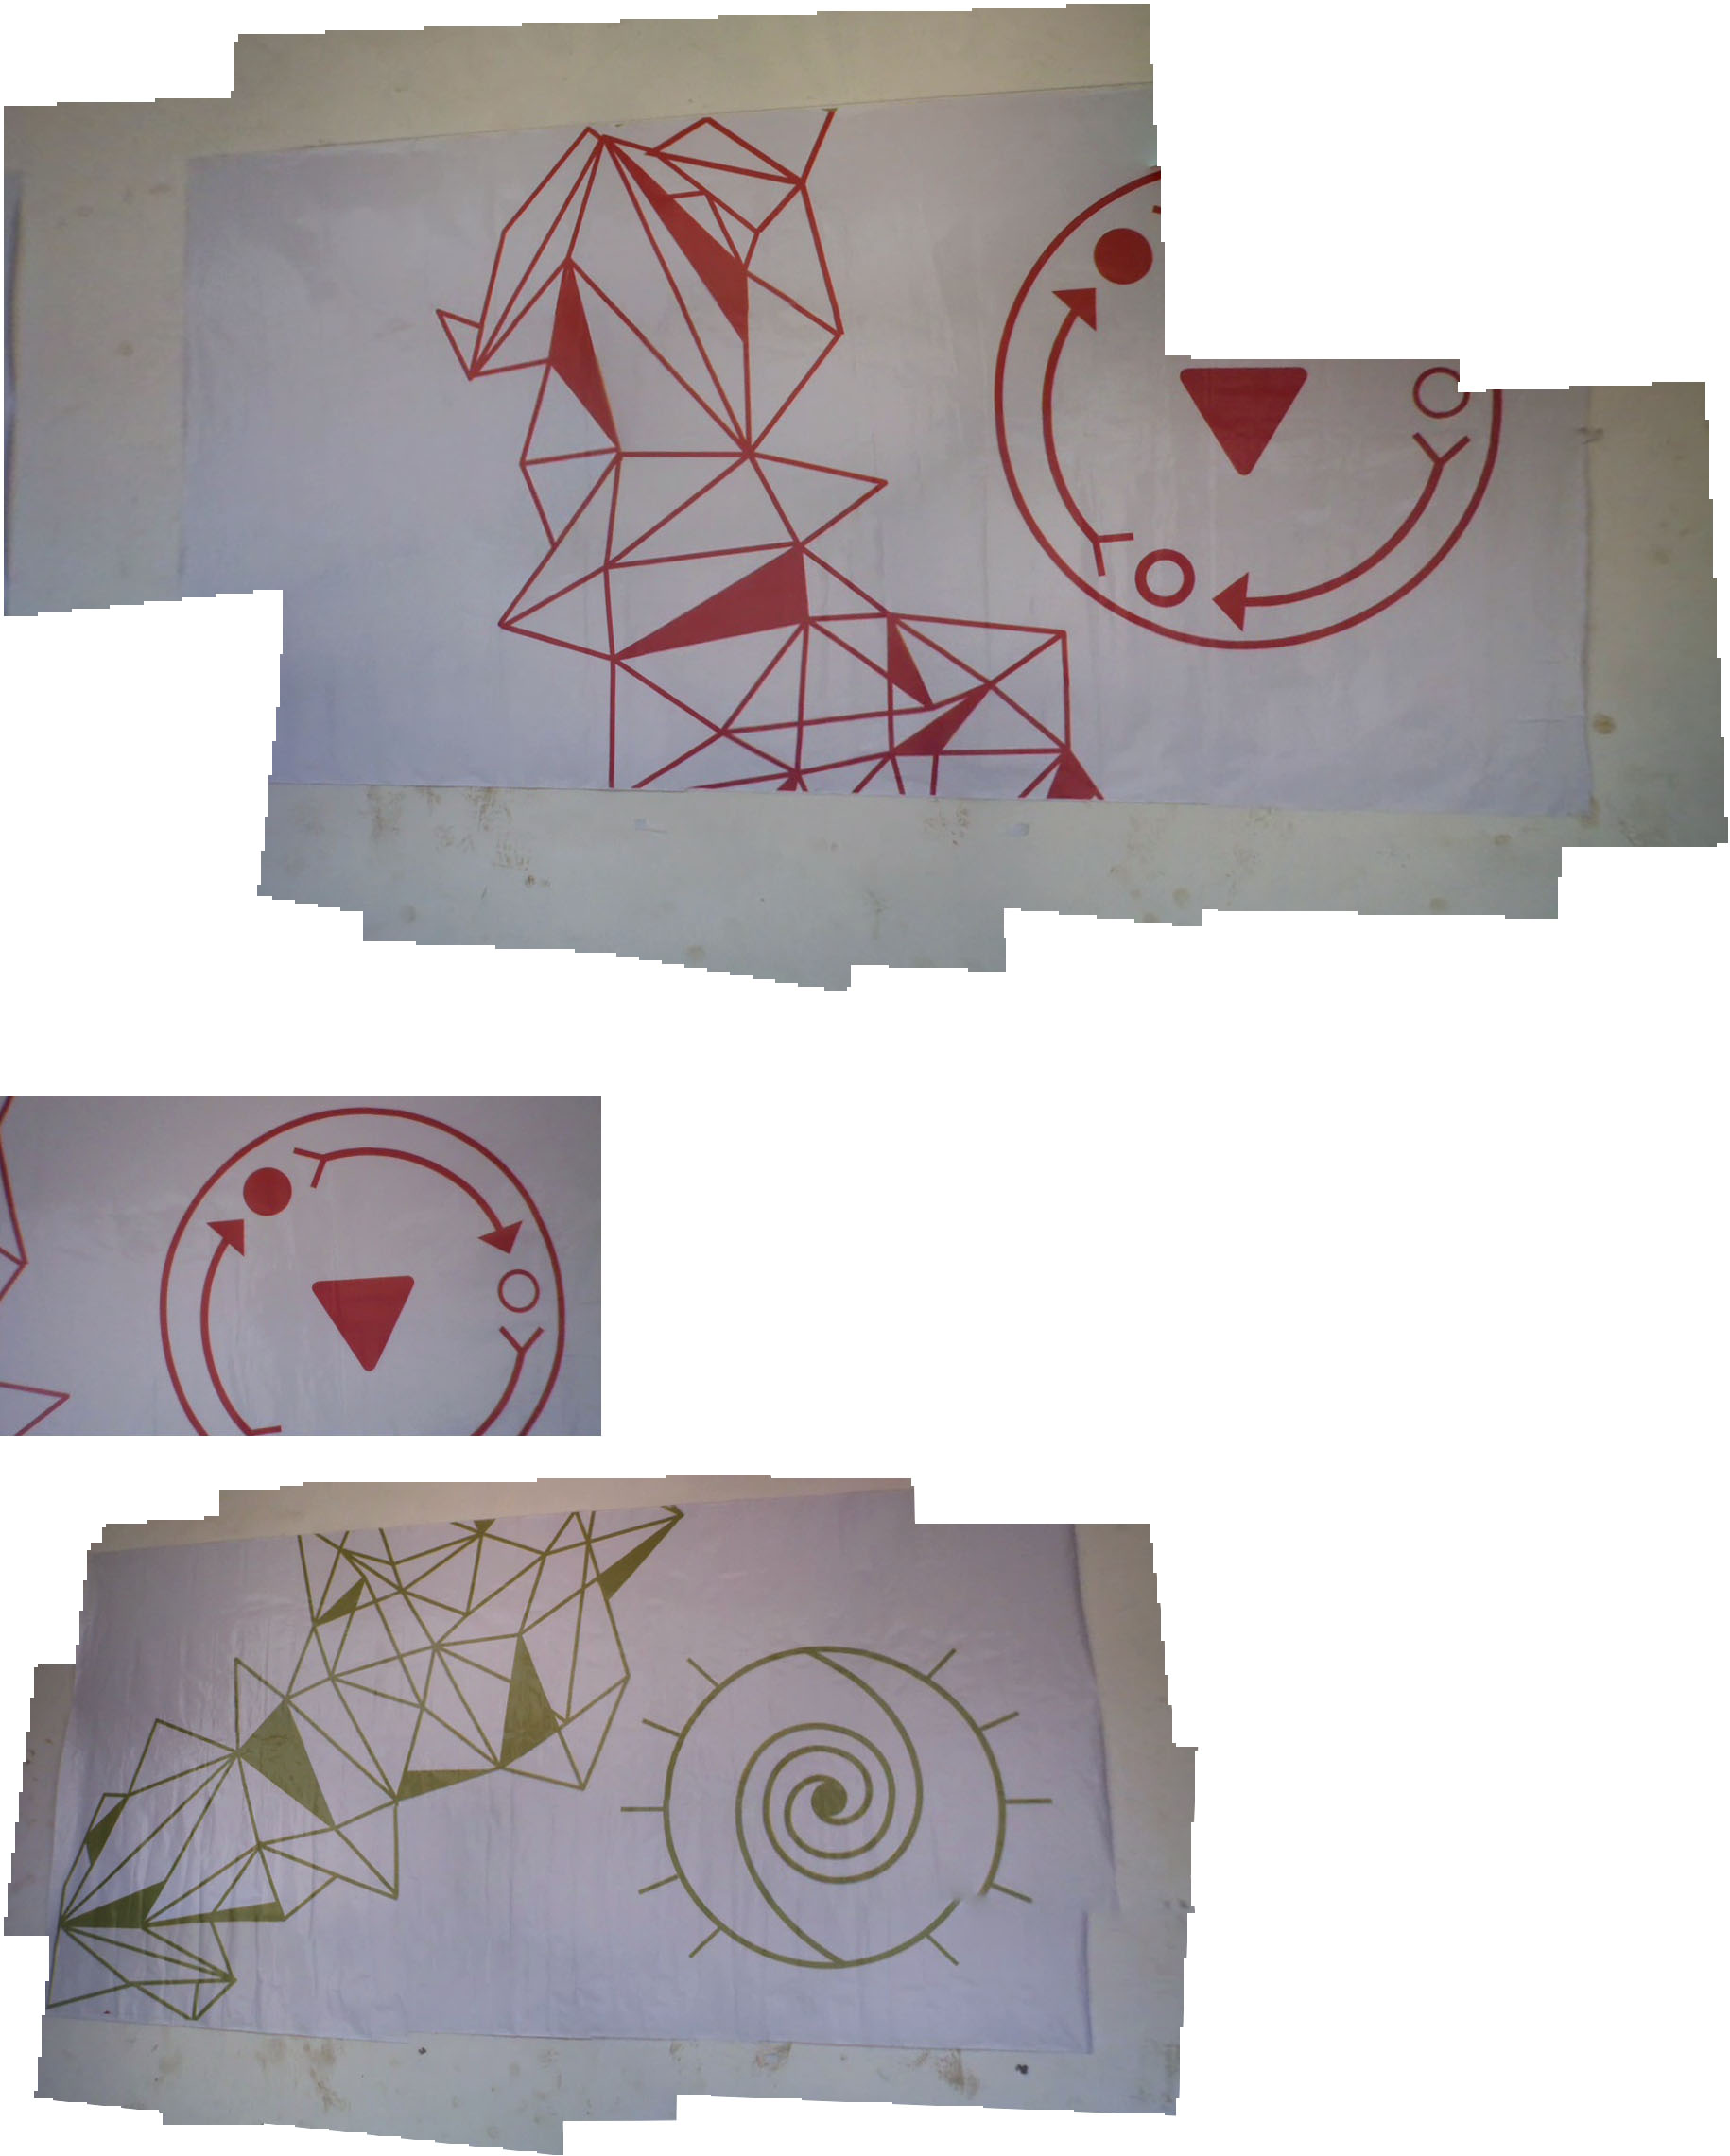
\includegraphics[width=\linewidth]{figures/green_red/photoshop_output.jpg}
\caption{Photoshop Result}
\end{subfigure}\\
\begin{subfigure}[b]{\textwidth}
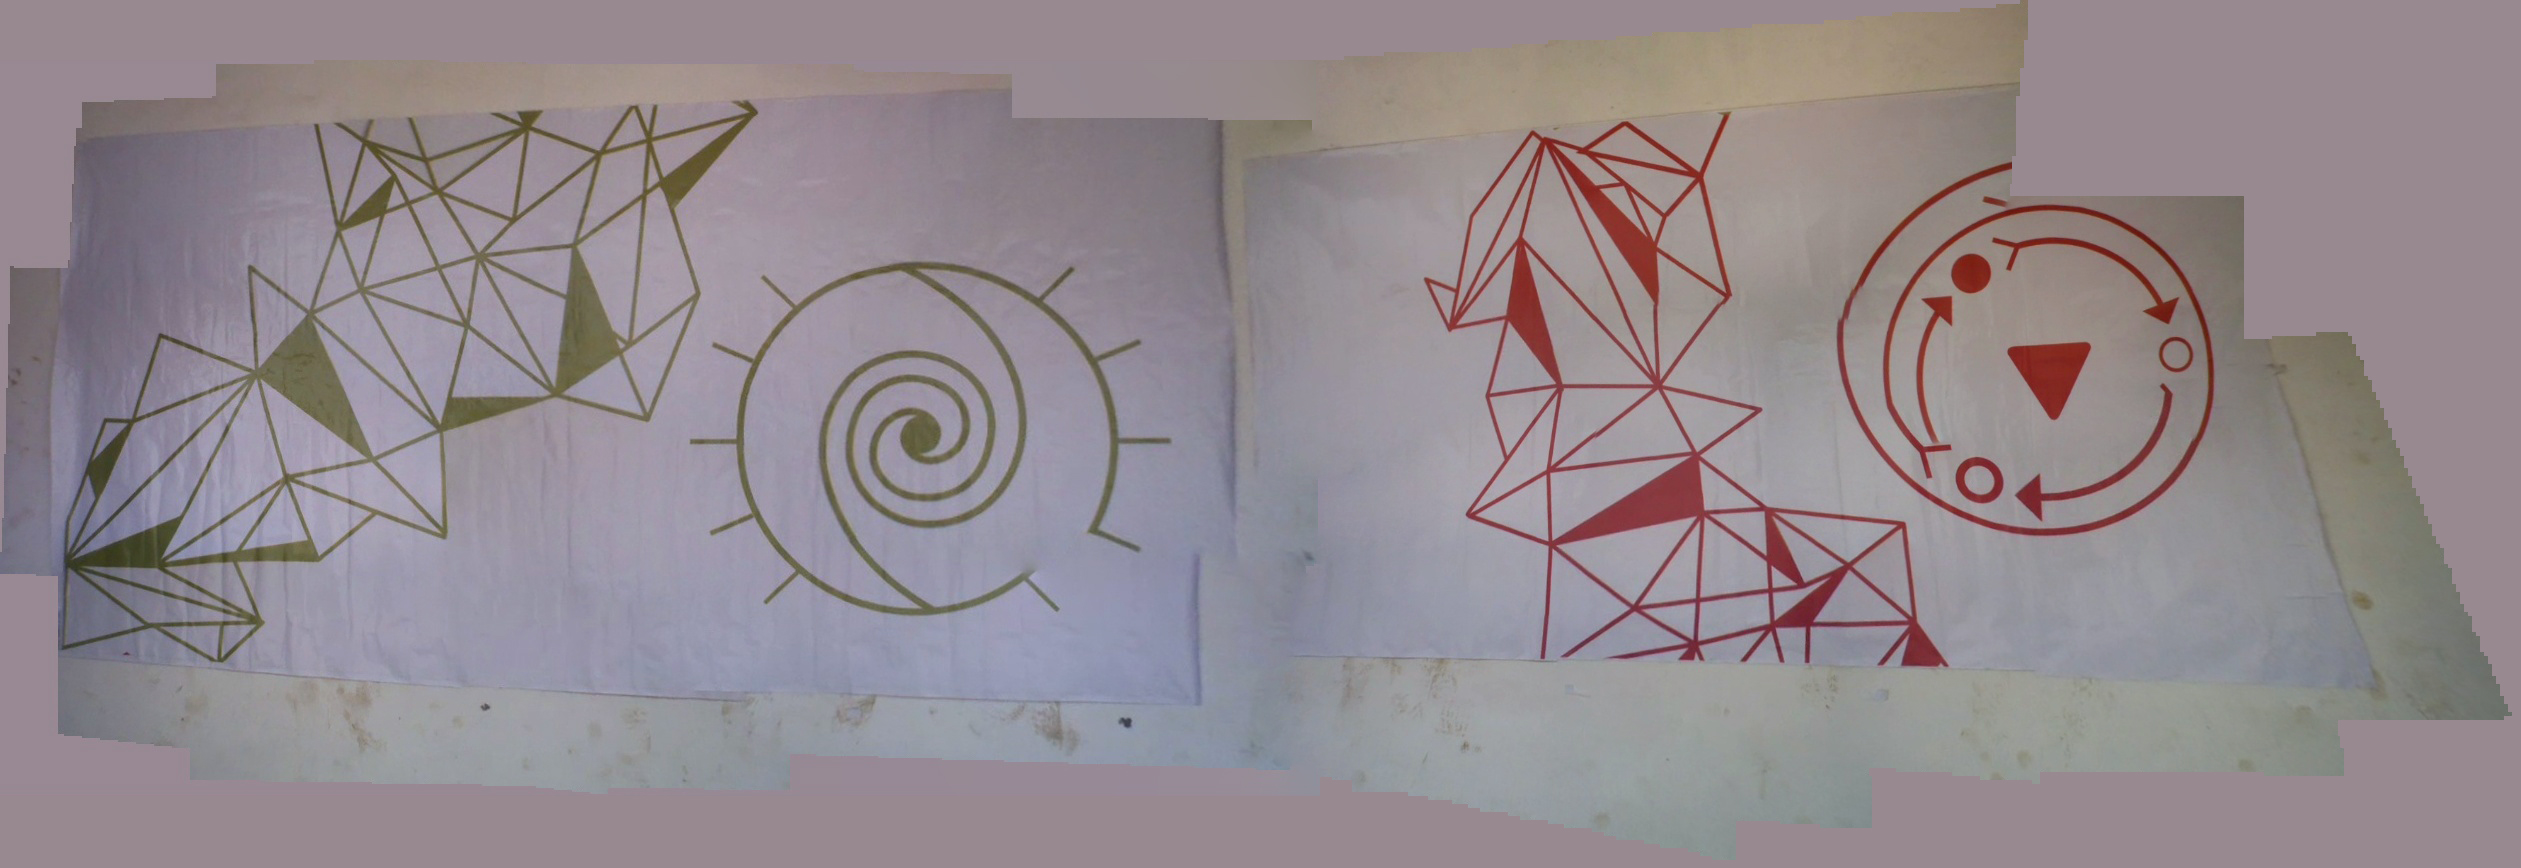
\includegraphics[width=\linewidth]{figures/green_red/our_result.jpg}
\caption{Our Result}
\end{subfigure}
\caption{Comparison of outputs of Autostich, Photoshop and our stitching
algorithm on the images selected of outdoor scene by our algorithm. Only our
output is able to shows individual panoramas at their respective location
approximately}
\label{fig:green_red_comparison}
\end{figure*}

Figure \ref{fig:green_red_comparison} shows the comparison of outputs of
state of the art stitchers with output of our algorithm.

\section{Concluding remarks}

In this paper, we have defined a new problem, that of computing a
mosaic of a planar scene with dead space.  Dead space relates to images
in an input stream where there are not enough features for traditional
mosaicing algorithms to stitch together a pleasing composite.  

Our solution to this problem is to use an autonomous quadcopter which
is capable of taking pictures.  The quadcopter has an inertial
measurement unit that is capable of outputting approximate
positions. Using this positional information, our algorithm selects an
``interesting'' subset of the video imagery.  This subset consists of
pictures taken with a ``moving'' camera; we reduce the resulting
problem of computing a mosaic by reduction to the stereo problem.  Our
method works on both indoor and outdoor scenes.

{\bf Future work} Controlling a consumer-focused inexpensive
quadcopter can be problematic; for instance the quadcopter could have
severe yaw and roll.  Vision based algorithms to control such
quadcopters might be quite useful.


\bibliographystyle{ieee}
\bibliography{egbib}
\end{document}
